%% abtex2-modelo-relatorio-tecnico.tex, v-1.9.7 laurocesar
%% Copyright 2012-2018 by abnTeX2 group at http://www.abntex.net.br/ 
%%
%% This work may be distributed and/or modified under the
%% conditions of the LaTeX Project Public License, either version 1.3
%% of this license or (at your option) any later version.
%% The latest version of this license is in
%%   http://www.latex-project.org/lppl.txt
%% and version 1.3 or later is part of all distributions of LaTeX
%% version 2005/12/01 or later.
%%
%% This work has the LPPL maintenance status `maintained'.
%% 
%% The Current Maintainer of this work is the abnTeX2 team, led
%% by Lauro César Araujo. Further information are available on 
%% http://www.abntex.net.br/
%%
%% This work consists of the files abntex2-modelo-relatorio-tecnico.tex,
%% abntex2-modelo-include-comandos and abntex2-modelo-references.bib
%%

% ------------------------------------------------------------------------
% ------------------------------------------------------------------------
% abnTeX2: Modelo de Relatório Técnico/Acadêmico em conformidade com 
% ABNT NBR 10719:2015 Informação e documentação - Relatório técnico e/ou
% científico - Apresentação
% ------------------------------------------------------------------------ 
% ------------------------------------------------------------------------

\documentclass[
  % -- opções da classe memoir --
  12pt,				% tamanho da fonte
  openright,			% capítulos começam em pág ímpar (insere página vazia caso preciso)
  twoside,			% para impressão em recto e verso. Oposto a oneside
  a4paper,			% tamanho do papel. 
  % -- opções da classe abntex2 --
  %chapter=TITLE,		% títulos de capítulos convertidos em letras maiúsculas
  %section=TITLE,		% títulos de seções convertidos em letras maiúsculas
  %subsection=TITLE,	% títulos de subseções convertidos em letras maiúsculas
  %subsubsection=TITLE,% títulos de subsubseções convertidos em letras maiúsculas
  % -- opções do pacote babel --
  english,			% idioma adicional para hifenização
  french,				% idioma adicional para hifenização
  spanish,			% idioma adicional para hifenização
  brazil,				% o último idioma é o principal do documento
  ]{abntex2}


% ---
% PACOTES
% ---
% ---- packs adicionais
\usepackage{lastpage}
\usepackage{xcolor}
\usepackage{listings}
\lstset{basicstyle=\ttfamily,
  showstringspaces=false,
  commentstyle=\color{red},
  keywordstyle=\color{blue}
}
\usepackage{hyperref}
\usepackage{caption}
\usepackage{subcaption}
\usepackage{adjustbox}
\usepackage{etoolbox}

% ---
% Pacotes fundamentais 
% ---
\usepackage{lmodern}			% Usa a fonte Latin Modern
\usepackage[T1]{fontenc}		% Selecao de codigos de fonte.
\usepackage[utf8]{inputenc}		% Codificacao do documento (conversão automática dos acentos)
\usepackage{indentfirst}		% Indenta o primeiro parágrafo de cada seção.
\usepackage{color}				% Controle das cores
\usepackage{graphicx}			% Inclusão de gráficos
\usepackage{microtype} 			% para melhorias de justificação
% ---

% ---
% Pacotes adicionais, usados no anexo do modelo de folha de identificação
% ---
\usepackage{multicol}
\usepackage{multirow}
% ---
  
% ---
% Pacotes adicionais, usados apenas no âmbito do Modelo Canônico do abnteX2
% ---
\usepackage{lipsum}				% para geração de dummy text
\usepackage{amssymb}
\usepackage{empheq,amsmath}
% ---

% ---
% Pacotes de citações
% ---
\usepackage[brazilian,hyperpageref]{backref}	 % Paginas com as citações na bibl
\usepackage[ieeetr]{abntex2cite}	% Citações padrão ABNT
\citebrackets[]

% --- 
% CONFIGURAÇÕES DE PACOTES
% --- 

% ---
% Configurações do pacote backref
% Usado sem a opção hyperpageref de backref
\renewcommand{\backrefpagesname}{Citado na(s) página(s):~}
% Texto padrão antes do número das páginas
\renewcommand{\backref}{}
% Define os textos da citação
\renewcommand*{\backrefalt}[4]{
  \ifcase #1 %
    Nenhuma citação no texto.%
  \or
    Citado na página #2.%
  \else
    Citado #1 vezes nas páginas #2.%
  \fi}%
% ---

% ---
% Informações de dados para CAPA e FOLHA DE ROSTO
% ---
\titulo{Implementações práticas de DSP e RF com GNURadio e HackRF One}
\autor{Jefferson da Silva Cândido}
\local{Uberlândia, Minas Gerais}
\data{\the\year}
\instituicao{%
  Universidade Federal de Uberlândia -- UFU
  \par
  Faculdade de Engenharia Elétrica
  \par
  Graduação em Engenharia Eletrônica e de Telecomunicações}
\tipotrabalho{Trabalho de Conclusão de Curso}
% O preambulo deve conter o tipo do trabalho, o objetivo, 
% o nome da instituição e a área de concentração 
\orientador{Dr. Antônio Cláudio Paschoarelli Veiga}

\preambulo{Trabalho apresentado na Universidade Federal de Uberlândia como requisito para conclusão do curso de graduação em Engenharia Eletrônica e de Telecomunicações.}
% ---

% ---
% Configurações de aparência do PDF final

% alterando o aspecto da cor azul
\definecolor{blue}{RGB}{41,5,195}

% informações do PDF
\makeatletter
\hypersetup{
      %pagebackref=true,
    pdftitle={\@title}, 
    pdfauthor={\@author},
      pdfsubject={\imprimirpreambulo},
      pdfcreator={LaTeX with abnTeX2},
    pdfkeywords={abnt}{latex}{abntex}{abntex2}{relatório técnico}, 
    colorlinks=true,       		% false: boxed links; true: colored links
      linkcolor=blue,          	% color of internal links
      citecolor=blue,        		% color of links to bibliography
      filecolor=magenta,      		% color of file links
    urlcolor=blue,
    bookmarksdepth=4
}
\makeatother
% --- 

% --- 
% Espaçamentos entre linhas e parágrafos 
% --- 

% O tamanho do parágrafo é dado por:
\setlength{\parindent}{1.3cm}

% Controle do espaçamento entre um parágrafo e outro:
\setlength{\parskip}{0.2cm}  % tente também \onelineskip

% ---
% compila o indice
% ---
\makeindex
% ---

% ----
% Início do documento
% ----
\begin{document}

% Seleciona o idioma do documento (conforme pacotes do babel)
\selectlanguage{brazil}

% Retira espaço extra obsoleto entre as frases.
\frenchspacing

% ----------------------------------------------------------
% ELEMENTOS PRÉ-TEXTUAIS
% ----------------------------------------------------------
\pretextual

% ---
% Capa
% ---
\imprimircapa
% ---

% ---
% Folha de rosto
% (o * indica que haverá a ficha bibliográfica)
% ---
\imprimirfolhaderosto
% ---

\begin{folhadeaprovacao}

  \begin{center}

    {\ABNTEXchapterfont\large\textsc{\imprimirautor}}

    {\ABNTEXchapterfont\Large\bfseries\imprimirtitulo}

  \end{center}

  \vspace{1cm}

  \hspace{.45\textwidth} \begin{minipage}{.45\textwidth}

    \imprimirpreambulo

  \end{minipage}

  \vspace{1cm}

  Trabalho aprovado. Uberlândia, 09 de dezembro de 2020

  %%%%%%%%%%%%%%%%%%%%%%%%%%

  %Assinaturas

  %%%%%%%%%%%%%%%%%%%%%%%%%%%%%%%%%%%%%%%%%%%%%%
  \assinatura{\textbf{\imprimirorientador} \\ Orientador}
  \assinatura{\textbf{Dr. Gilberto Arantes Carrijo} \\ Convidado 1}
  \assinatura{\textbf{Dr. Éderson Rosa da Silva} \\ Convidado 2}
  %%%%%%%%%%%%%%%%%%%%%%%%%%%%%%%%%%%%%%%%%%%%%%%%%%%

  %%%%%%%%%%%%%%%%%%%%%%%%%%%%%%%%%%%%%%%%%%%%%%%%%%%
  \begin{center}
    \vfill
    {\large\imprimirlocal}
    \par
    {\large\imprimirdata}

  \end{center}
\end{folhadeaprovacao}
%%%%%%%%%%%%%%%%%%%%%%%%%%%%%%%%%

%Fim da folha de aprovação
%%%%%%%%%%%%%%%%%%%%%%%%%%%%%%%

%%%%%%%%%%%%%%%%%%%%%%%%%%%%%%%%%
% Início da dedicatória - Elemento opcional
%%%%%%%%%%%%%%%%%%%%%%%%%%%%%%%%%%%%%%%%%%%%%%%%%%%%%%%%%%%
\begin{dedicatoria}
  \vspace*{\fill}
  Este trabalho é dedicado à minha mãe, Maria Aparecida da Silva, que sempre me foi exemplo de obstinação, diligência e honradez.
  \vspace*{\fill}

\end{dedicatoria}
%%%%%%%%%%%%%%%%%%%%%%%%%%%%%%%%%%%%%%%%%%%%%%%%%%

% Fim da dedicatória
%%%%%%%%%%%%%%%%%%%%%%%%%%%%%%%%%%%%%%%%%%%%%%%%%%

% ---
% Agradecimentos
% ---
\begin{agradecimentos}
  Agradeço primeiramente a minha família por ter apoiado e viabilizado todo esse processo de
  aprendizado.

  Sou grato pela liberdade e confiança dispensada pelo meu orientador, professor Dr. Antônio
  Cláudio Paschoarelli Veiga.

  Aos professores que contribuíram para o cumprimento dessa jornada.

  À Universidade Federal de Uberlândia por cumprir veementemente com o seu papel de formação de
  cidadãos.

  Aos colegas do laboratório de Redes de Computadores e Telecomunicações, William, Daniel e Caio
  por todo apoio e amizade.

  Agradeço também a todas as entidades que estiveram presentes durante minha formação, com destaques
  para o Diretório Acadêmico da Faculdade de Engenharia Elétrica e ao Laboratório de Automação,
  Sistemas Eletrônicos e Controle (LASEC), que muito auxiliaram no meu desenvolvimento profissional
  e de liderança.

\end{agradecimentos}
% ---

%%%%%%%%%%%%%%%%%%%%%%% 
% Início da epígrafe - opcional 
%%%%%%%%%%%%%%%%%%%%%%%%%%%%%%%%%%%%%%%%%%%%%%%%%%%%%%%%%%%%%% 
\begin{epigrafe}
  \vspace*{\fill}
  \begin{flushright}
    \textit{``Messages and the corresponding signals are points in two "function spaces", and the
      modulation process is a mapping of one space into other.''\\ (Claude E. Shannon)}
  \end{flushright}
\end{epigrafe}
%%%%%%%%%%%%%%%%%%%%%%%%%%%%%%%%%%%%%%%%%%%%%%%%%%%%%%%%%%%%%%%%% 
% Fim da epígrafe - opcional 
%%%%%%%%%%%%%%%%%%%%%%%%%%%%%%%%%%%%%%%%%%%%%%%%%%%%%%%%%%%%%%

% ---
% RESUMO
% ---

% resumo na língua vernácula (obrigatório)
\setlength{\absparsep}{18pt} % ajusta o espaçamento dos parágrafos do resumo
\begin{resumo}

  Este é um trabalho introdutório e prático de pesquisa direcionado às áreas de processamento digital de sinais e transmissão e recepção de sinais de radiofrequência.
  O objetivo é que ele se torne um pontapé inicial para que estudantes de engenharia eletrônica e de telecomunicações possam ter um primeiro contato prático com
  técnicas de processamento digital de sinais aplicadas a partir de um sistema de rádio definido por software.

  A proposta de realização dos experimentos conta com a  utilização de métodos e técnicas de programação em C++/Python para a construção de módulos e blocos de processamento
  de sinais em conjunto ao uso de um \textit{hardware} (o SDR \textit{HackRF One}) dedicado ao propósito de ser a interface entre um computador e o \textit{frontend} de radiofrequência.

  No decorrer do trabalho são demonstrados detalhes de implementação, comunicação entre o \textit{hardware} e provisionamento do ambiente e das ferramentas de
  \textit{software} necessárias para a sua realização. Todos os esforços direcionados resultaram no êxito da demonstração do uso prático da ferramenta GNURadio, assim como
  a possibilidade de que o engenheiro também atue como um desenvolvedor, o que traz ganhos extremamente benéficos ao seu aprendizado e especialização profissional, além da
  possibilidade de aplicação dos conceitos teóricos adquiridos sobre sinais e sistemas, processamento digital de sinais, programação de sistemas de alta criticidade, sistemas
  de comunicações, modulação e demodulação e etc \ldots

  \noindent
  \textbf{Palavras-chaves}: rádio, software, gnuradio, hackrf, sdr.
\end{resumo}

% Resumo em inglês

\begin{resumo}[Abstract]
  \begin{otherlanguage*}{english}
    This is an introductory and practical research work aimed at the areas of digital signal processing and the
    transmission and reception of radio frequency signals. The goal is that it becomes a starting point for
    students of electronic and telecommunications engineering to have a first practical contact with digital
    signal processing techniques applied from a software-defined radio system.

    The proposal for carrying out the experiments relies on the use of programming methods and techniques in
    C++/Python for the construction of modules and signal processing blocks together with the use of a
    \textit{hardware} (SDR \textit{HackRF One}) dedicated to the purpose of being the interface between a
    computer and the radio frequency \textit{frontend}.

    During the work, details of implementation, communication between \textit{hardware} and provisioning of
    the environment and the \textit{software} tools necessary for its realization are demonstrated. All directed
    efforts resulted in the successful demonstration of the practical use of the GNURadio tool, as well as the
    possibility that the engineer also acts as a developer, which brings extremely beneficial gains to his
    learning and professional specialization, in addition to the possibility of applying of the theoretical
    concepts acquired about signals and systems, digital signal processing, programming of high criticality
    systems, communication systems, modulation and demodulation and etc \ldots

    \vspace{\onelineskip}
    \noindent
    \textbf{Keywords}: radio, software, gnuradio, hackrf, sdr.
  \end{otherlanguage*}
\end{resumo}
% ---

% ---
% inserir lista de ilustrações
% ---
\pdfbookmark[0]{\listfigurename}{lof}
\listoffigures*
\cleardoublepage
% ---

% ---
% inserir lista de tabelas
% ---
\pdfbookmark[0]{\listtablename}{lot}
\listoftables*
\cleardoublepage
% ---

% ---
% inserir lista de abreviaturas e siglas
% ---
\begin{siglas}

  \item[ADC]         \textit{Analog to Digital Converter}
  \item[ARM]        \textit{Advanced RISC}
  \item[BW]         \textit{Bandwidth}
  \item[CLI]        \textit{Command Line Interface}
  \item[DAC]        \textit{Digital to Analog Converter}
  \item[DSP]        \textit{Digital Signal Processing}
  \item[FFT]        \textit{Fast Fourier Transform}
  \item[FIR]        \textit{Finite Impulse Response}
  \item[FM]         \textit{Frequency Modulation}
  \item[FSF]        \textit{Free Software Foundation}
  \item[GNU]        \textit{GNU's Not Unix}
  \item[GPG]        \textit{GNU Privacy Guard}
  \item[GPLv3]      \textit{General Public License version 3}
  \item[GPSDO]      \textit{GPS Disciplined Oscillator}
  \item[GRC]        \textit{GNURadio Companion}
  \item[GUI]        \textit{Graphical User Interface}
  \item[LPF]        \textit{Low-Pass Filter}
  \item[OCXO]       \textit{Oven Controlled Crystal Oscillator}
  \item[OOT]        \textit{Out of Tree}
  \item[SDK]        \textit{Software Development Kit}
  \item[SDR]        \textit{Software-defined Radio}
  \item[SELinux]    \textit{Security-Enhanced Linux}
  \item[SPC]        \textit{Super Privileged Container}
  \item[STDIN]      \textit{Standard Input}
  \item[TCXO]       \textit{Temperature Compensated Crystal Oscillator}
  \item[TDD]        \textit{Test Driven Development}
  \item[TTY]        \textit{TeleTYpewriter}

\end{siglas}
% ---

% ---
% inserir lista de símbolos
% ---
\begin{simbolos}
  \item[$ R_b $] Taxa de bits [bits/s]
  \item[$ R_s $] Taxa de símbolos [amostras/s]
  \item[$ dB $] Decibel
  \item[$ P $] Potência [W]
  \item[$f$] Frequência [Hz]
  \item[$\omega$] Frequência angular [rad/s]
  \item[$f_s$] Frequência de amostragem [Hz]
\end{simbolos}
% ---

% ---
% inserir o sumario
% ---
\pdfbookmark[0]{\contentsname}{toc}
\tableofcontents*
\cleardoublepage
% ---

% ----------------------------------------------------------
% ELEMENTOS TEXTUAIS
% ----------------------------------------------------------
\textual

% ----------------------------------------------------------
% Introdução (exemplo de capítulo sem numeração, mas presente no Sumário)
% ----------------------------------------------------------
\chapter*[Introdução]{Introdução}
\addcontentsline{toc}{chapter}{Introdução}

O processamento digital de sinais que é conhecido por engenheiros atualmente começou a florescer por volta dos anos 1960 \cite{hayes:1999} passando por uma evolução
dramática até alcançar solidez em técnicas e implementações. O cenário atual que o mundo se encontra é altamente favorável para que estudantes de engenharia
direcionem seus esforços para esta área, pois o processo de transformação digital da indústria e da sociedade está ocorrendo de forma acelerada
\cite{ebert:digital_transformation} mantendo alta a demanda por profissionais com habilidades técnicas correlatas.

Os grandes aliados do engenheiro na execução de seus trabalhos estão diretamente relacionados com a sua capacidade de descobrir e aplicar ferramentas que facilitem a execução de suas
tarefas e a geração de relatórios e métricas que auxiliem em diagnósticos e na tomada de decisões que impactam os negócios que ele está envolvido, seja como funcionário ou como empreendedor.
Dentre as principais ferramentas que o engenheiro pode ter ao seu lado, está o uso de boas práticas no que tange o desenvolvimento de \textit{software} e, mais especificamente para este trabalho,
está a ferramenta GNURadio que vem como uma proposta livre de integração e multi-disciplinaridade dentro das áreas estudadas por engenheiros em eletrônica e telecomunicações.

Para utilizar o \textit{software} escrito utilizando o GNURadio além das simulações, o engenheiro precisa de um \textit{hardware}, chamado SDR (\textit{Software-defined Radio}), capaz de receber este \textit{software} fazer as devidas
conversões de frequência e transmitir/receber o sinal de radiofrequência desejado. As vantagens na utilização do SDR como o reuso de \textit{hardware} e a utilização de níveis mais altos de abstração do \textit{software} como também algumas desvantagens (desempenho inferior
se comparado a \textit{hardware}'s dedicados,  problemas  de  interoperabilidade e segurança) devem sempre ser avaliados para cada projeto \cite{sbrc:minicurso_gnuradio}

Um dos diferenciais alcançados durante o desenvolvimento dessa pesquisa foi a utilização de \textit{container}'s para o isolamento do ambiente de desenvolvimento de \textit{software}, o que
flexibiliza o processo de criação, sendo que o impacto esperado é incentivar que outros estudantes também apliquem seus conhecimentos teóricos sobre processamento digital de sinais
utilizando as ferramentas e boas práticas que aqui serão mencionadas.

O objetivo principal deste trabalho será trazer a visão de um estudante de engenharia eletrônica e de telecomunicações sobre o contato inicial com o desenvolvimento de aplicações de rádio
definido por \textit{software} utilizando o GNURadio para a realização do processamento digital de sinais.

% ----------------------------------------------------------
% PARTE - preparação do ambiente de desenvolvimento
% ----------------------------------------------------------
\part{Preparações}

\chapter{Hardware}

Neste capítulo são abordados os dispositivos de \textit{hardware} utilizados no desenvolvimento deste trabalho, trazendo brevemente um comparativo de quais
podem ser encontrados no mercado atualmente e quais as especificações técnicas disponibilizadas por alguns fabricantes.

Basicamente, é necessário um dispositivo \textit{host} (arquiteturas \textbf{x86\_64} ou \textbf{amd64}, \textbf{armhf} e \textbf{arm64}/\textbf{aarch64}, por exemplo),
preferencialmente com alguma distribuição \textit{Linux} e o \textit{GNURadio-companion} instalados, uma placa de circuito impresso do sistema de rádio
definido por \textit{software} contendo algum cabo para comunicação com o computador \textit{host} (normalmente USB 2.0/3.0), as antenas para transmissão e/ou recepção
e algum oscilador (TCXO (\textit{Temperature Compensated Crystal Oscillator}), OCXO (\textit{Oven Controlled Crystal Oscillator}), GPSDO (\textit{GPS Disciplined Oscillator}), etc...)
caso a aplicação exija sincronismo por \textit{clock} externo.

Com relação ao computador utilizado, trata-se de um notebook de arquitetura \textbf{amd64} com 8 GB de memória DDR3 e processador Intel® Core™ i7 de terceira geração com quatro núcleos e
3.0 GHz de \textit{clock} conforme estatísticas retiradas do próprio sistema operacional e mostradas na Fig. \ref{fig:host_pc_stats}.

\begin{figure}[!htb]
  \centering
  \caption{Configurações de CPU e memória do computador utilizado.}
  \includegraphics[width = \linewidth]{figures/host-pc/stats.png}
  Fonte: Elaborado pelo autor.
  \label{fig:host_pc_stats}
\end{figure}

\section*{Avaliação de SDR's}

Para o sistema de rádio definido por \textit{software} primeiramente foi realizada uma pesquisa de mercado para avaliar quais os SDR's disponíveis e quais
\textit{feature's} cada um oferece. Pontos importantes a serem observados antes de efetuar a compra de um SDR são: se ele pode atuar apenas como receptor
(RX) ou como receptor e trasmissor (RX/TX), qual a faixa de frequência de atuação, a largura de banda máxima e a resolução do ADC/DAC (número de \textit{bits} por amostra),
qual o suporte a nível de \textit{software} e qual o custo do investimento. Entre os dispostivos apenas receptores, destacaram-se o RTL-SDR, o AirSpy Mini e o SDRplay RSPduo,
os quais atuam até a casa de 2 GHz aproximadamente com laguras de banda máximas variando entre 3 MHz e 10 MHz. Com relação aos SDR's RX/TX foram considerados
o LimeSDR Mini, BladeRF, \textit{HackRF One}, Ettus USRP B210 e o Adalm PlutoSDR e todos podem ser utilizados com largura de banda de pelo menos 20 MHz e podendo variar
entre 1 MHz e 6 GHz no domínio da frequência.

O resumo dos principais SDR's que podem ser encontrados no mercado é mostrado na Tabela \ref{table:SDR_comparison}, com preços em dólares cotados \textit{online} através do site \href{https://pt.aliexpress.com}{https://pt.aliexpress.com}
e também dos própiros fabricantes \href{https://www.sdrplay.com/rspduo/}{SDRplay}, \href{https://www.analog.com/en/design-center/evaluation-hardware-and-software/evaluation-boards-kits/adalm-pluto.html}{Analog Devices} (Adalm Pluto),
\href{https://www.nuand.com/bladerf-1/}{Nuand} (BladeRF) e \href{https://www.ettus.com/all-products/ub210-kit/}{Ettus} (USRP B210). O SDR escolhido para este trabalho foi o \textit{HackRF One}, que será abordado com mais detalhes na próxima seção.

\begin{table}[!htb]
  \caption{Comparativo de SDR's a nível de \textit{hardware} e custo de investimento.}
  \centering
  \resizebox{\linewidth}{!}{
    \begin{tabular}{|l|r|r|r|r|r|r|}
      \hline
                                          & \multicolumn{1}{c|}{\textbf{\begin{tabular}[c]{@{}c@{}}Faixa\\ de\\ frequência\end{tabular}}} & \multicolumn{1}{c|}{\textbf{\begin{tabular}[c]{@{}c@{}}Largura\\ de banda\\ máxima\end{tabular}}} & \multicolumn{1}{c|}{\textbf{\begin{tabular}[c]{@{}c@{}}RX/\\ TX\end{tabular}}} & \multicolumn{1}{c|}{\textbf{\begin{tabular}[c]{@{}c@{}}Half /\\ Full Duplex\end{tabular}}} & \multicolumn{1}{c|}{\textbf{\begin{tabular}[c]{@{}c@{}}Resolução\\ do ADC\end{tabular}}} & \multicolumn{1}{c|}{\textbf{\begin{tabular}[c]{@{}c@{}}Preço\\ (US\$)\end{tabular}}} \\ \hline
      \textbf{RTL-SDR}                    & \begin{tabular}[c]{@{}r@{}}500 kHz\\ a\\ 1766 MHz\end{tabular}                               & 3 MHz                                                    & RX                                                       & -                                                        & 8 bits                                                   & $\sim$25,00                                              \\ \hline
      \textbf{RSPduo}                     & \begin{tabular}[c]{@{}r@{}}1 kHz\\ a\\ 2 GHz\end{tabular}                               & 10 MHz                                                   & RX                                                       & -                                                        & 14 bits                                                  & $\sim$260,00                                             \\ \hline
      \textbf{\begin{tabular}[c]{@{}l@{}}AirSpy\\ Mini\end{tabular}} & \begin{tabular}[c]{@{}r@{}}24 Hz\\ a\\ 1.7 GHz\end{tabular}                               & 6 MHz                                                    & RX                                                       & -                                                        & até 16 bits                                              & $\sim$150,00                                             \\ \hline
      \textbf{\begin{tabular}[c]{@{}l@{}}USRP\\ B200/\\ B210\end{tabular}} & \begin{tabular}[c]{@{}r@{}}70 MHz\\ a\\ 6 GHz\end{tabular}                               & 56 MHz                                                   & \begin{tabular}[c]{@{}r@{}}RX/\\ TX\end{tabular}                               & Full Duplex                                              & 12 bits                                                  & \begin{tabular}[c]{@{}r@{}}a partir\\ de 890,00\end{tabular}                               \\ \hline
      \textbf{PlutoSDR}                   & \begin{tabular}[c]{@{}r@{}}325 MHz\\ a\\ 3.8 GHz\end{tabular}                               & 20 MHz                                                   & \begin{tabular}[c]{@{}r@{}}RX/\\ TX\end{tabular}                               & Full Duplex                                              & 12 bits                                                  & 249,00                                                   \\ \hline
      \textbf{\begin{tabular}[c]{@{}l@{}}LimeSDR\\ Mini\end{tabular}} & \begin{tabular}[c]{@{}r@{}}10 MHz\\ a\\ 3.5 GHz\end{tabular}                               & 30 MHz                                                   & \begin{tabular}[c]{@{}r@{}}RX/\\ TX\end{tabular}                               & Full Duplex                                              & 12 bits                                                  & \begin{tabular}[c]{@{}r@{}}de 300,00\\ a 350,00\end{tabular}                               \\ \hline
      \textbf{BladeRF}                    & \begin{tabular}[c]{@{}r@{}}300 MHz\\ a\\ 3.8 GHz\end{tabular}                               & 40MHz                                                    & \begin{tabular}[c]{@{}r@{}}RX/\\ TX\end{tabular}                               & Full Duplex                                              & 12 bits                                                  & \begin{tabular}[c]{@{}r@{}}a partir\\ de 720,00\end{tabular}                               \\ \hline
      \textbf{HackRF}                     & \begin{tabular}[c]{@{}r@{}}1 MHz\\ a\\ 6 GHz\end{tabular}                               & 20 MHz                                                   & \begin{tabular}[c]{@{}r@{}}RX/\\ TX\end{tabular}                               & Half Duplex                                              & 8 bits                                                   & \begin{tabular}[c]{@{}r@{}}a partir\\ de 70,00\end{tabular}                               \\ \hline
    \end{tabular}
  }
  \label{table:SDR_comparison}
\end{table}

\subsection*{HackRF One}

% HACKRF: https://pt.aliexpress.com/item/32889992261.html

O \textit{HackRF One} é um SDR com \textit{hardware} de código aberto que foi desenvolvido pelo pesquisador em segurança de redes sem fio, Michael Ossmann. Trata-se de um transceptor \textit{half-duplex}
com largura de banda máxima de 20 MHz (BW - \textit{Bandwidth}) preparado para atuar em uma grande faixa de frequências que vão de 1 MHz a 6 GHz, possibilitando o processamento de até 20 milhões de amostras por
segundo (tendo 8 bits por amostra em quadratura - sinais I/Q com 8 bits para o I e 8 bits para o Q) recebidas ou transmitidas por meio de uma antena fixada em seu conector SMA fêmea, de
forma que o ganho - de recepção (RX) ou de transmissão (TX) - é configurável pelo \textit{software} utilizado, que neste caso é o GNURadio. O \textit{HackRF One} é alimentado pela tensão VCC fornecida
pela porta de comunicação USB 2.0, a qual também possibilita que o SDR transmita até 40 MB por segundo (20 milhões de amostras de 2 bytes a cada segundo).

Em quinze de maio de dois mil e quinze, Michael Ossmann publicou que seu SDR é capaz de operar em frequências menores que 10 MHz \cite{HACKRF-1mhz}, reafirmando a faixa de operação do \textit{HackRF One}.
A potência máxima de transmissão do \textit{HackRF One} varia de acordo com a faixa de frequência de operação e é suficiente para a realização de testes de curto alcance. Para recepção, o máximo de
potência fica na ordem de -5 dBm e exceder este valor pode resultar em danos permanentes ao \textit{HackRF One} \cite{HACKRF-hardware-receive-power}.

Os valores apresentados a seguir, aproximados, estão relacionados à potência de transmissão do \textit{HackRF One} e foram coletados e disponibilizados pelo fabricante \cite{HACKRF-hardware-transmit-power}:

\begin{itemize}
  \item[$-$] 1 MHz a 10 MHz: 5 dBm a 15 dBm (3 mW a 30 mW) - crescente com a frequência;
  \item[$-$] 10 MHz a 2150 MHz: 15 dBm a 5 dBm (30 mW a 3 mW) - decrescente com a frequência;
  \item[$-$] 2150 MHz a 2750 MHz: 13 dBm a 15 dBm (20 mW a 30 mW) - tendência de crescimento/decrescimento não informada pelo fabricante;
  \item[$-$] 2750 MHz a 4000 MHz: de 5 dBm a 0 dBm (3 mW a 1 mW) - decrescente com a frequência;
  \item[$-$] 4000 MHz a 6000 MHz: de 0 dBm a -10 dBm (1 mW a 0.1 mW) - decrescente com a frequência.
\end{itemize}

A Fig. \ref{fig:hackrf_block_diagram} ilustra o diagrama de blocos simplificado do \textit{HackRF One}. Por se tratar de um equipamento que lida com radiofrequência, o uso do \textit{HackRF One} deve estar dentro das observações legais da região em que for aplicado. No Brasil é importante que o
engenheiro esteja atento às regras reguladas pela Agência Nacional de Telecomunicações, ANATEL, como por exemplo a Resolução nº 716, de 31 de outubro de 2019 em que foi aprovado o plano de
atribuição, destinação e distribuição de faixas de frequências no Brasil (PDFF). O Anexo \ref{attachment:freq_range_brasil} contém o quadro de atribuição de faixas de frequências no Brasil, edição de 2019.

\begin{figure}[!htb]
  \centering
  \caption{Diagrama de blocos simplificado do \textit{HackRF One}.}
  \includegraphics[width = \linewidth, page=1, clip=true]{attachments/hackrf_SDR_diagram}
  Fonte: Elaborado pelo autor com base na documentação fornecida pelo fabricante \cite{HACKRF-hardware-components}.
  \label{fig:hackrf_block_diagram}
\end{figure}

O \textit{kit} que foi adquirido no site \href{https://pt.aliexpress.com}{https://pt.aliexpress.com} veio com uma placa de circuito impresso do SDR \textit{HackRF One}, um oscilador TCXO,
uma antena telescópica (banda passante de 40 MHz a 6 GHz), uma antena omnidirecional (para recepção de sinais GSM, 3G e 4G), um cabo USB e peças de acrílico para montagem do \textit{kit}. As fotos da Fig.
\ref{fig:hack_rf_hdk} foram tiradas após a montagem do \textit{kit} e os diagramas esquemático e de montagem referentes ao projeto foram anexados a este trabalho (Anexos \ref{attachment:hackrf-one-schematic-1} a \ref{attachment:hackrf-one-assembly}).

% \subsubsection*{ANTENA}

% % https://pt.dhgate.com/product/12dbi-high-gain-omni-directional-sma-male/429542258.html

% Inscrição:
% A antena é ótimo para veículos / automóvel / caminhão / uso van. Montado em uma superfície mental. E é funcionado como uma antena de alto ganho ao ar livre.

% Especificações:
% gama de frequência: 700 MHz-2700 MHz
% VSWR: menor ou igual a 1.5
% Ganho: 12dB
% impedância de entrada: 50 Ohm
% cabo coaxial: RG174 (3mm de diâmetro)
% comprimento do fio: 3M
% Tipo de conector: SMA-J

% Suporta todas as transportadoras que transmitem as seguintes bandas de frequência:
% 700-800 MHz 4.5dB
% 824-894 MHz 5dB
% 880-960 MHz 5dB
% 1710-1880 MHz 9.5dB
% 1850-1990 MHz 9.5dB
% 2110-2170 MHz 10dB
% 2500 $\sim$ 2700 MHz 12dB

% Incluído no Pacote:
% 1 x Mount Magnet Antena

\newpage
\begin{figure}[!htb]
  \centering
  \begin{subfigure}[b]{0.45\linewidth}
    \centering
    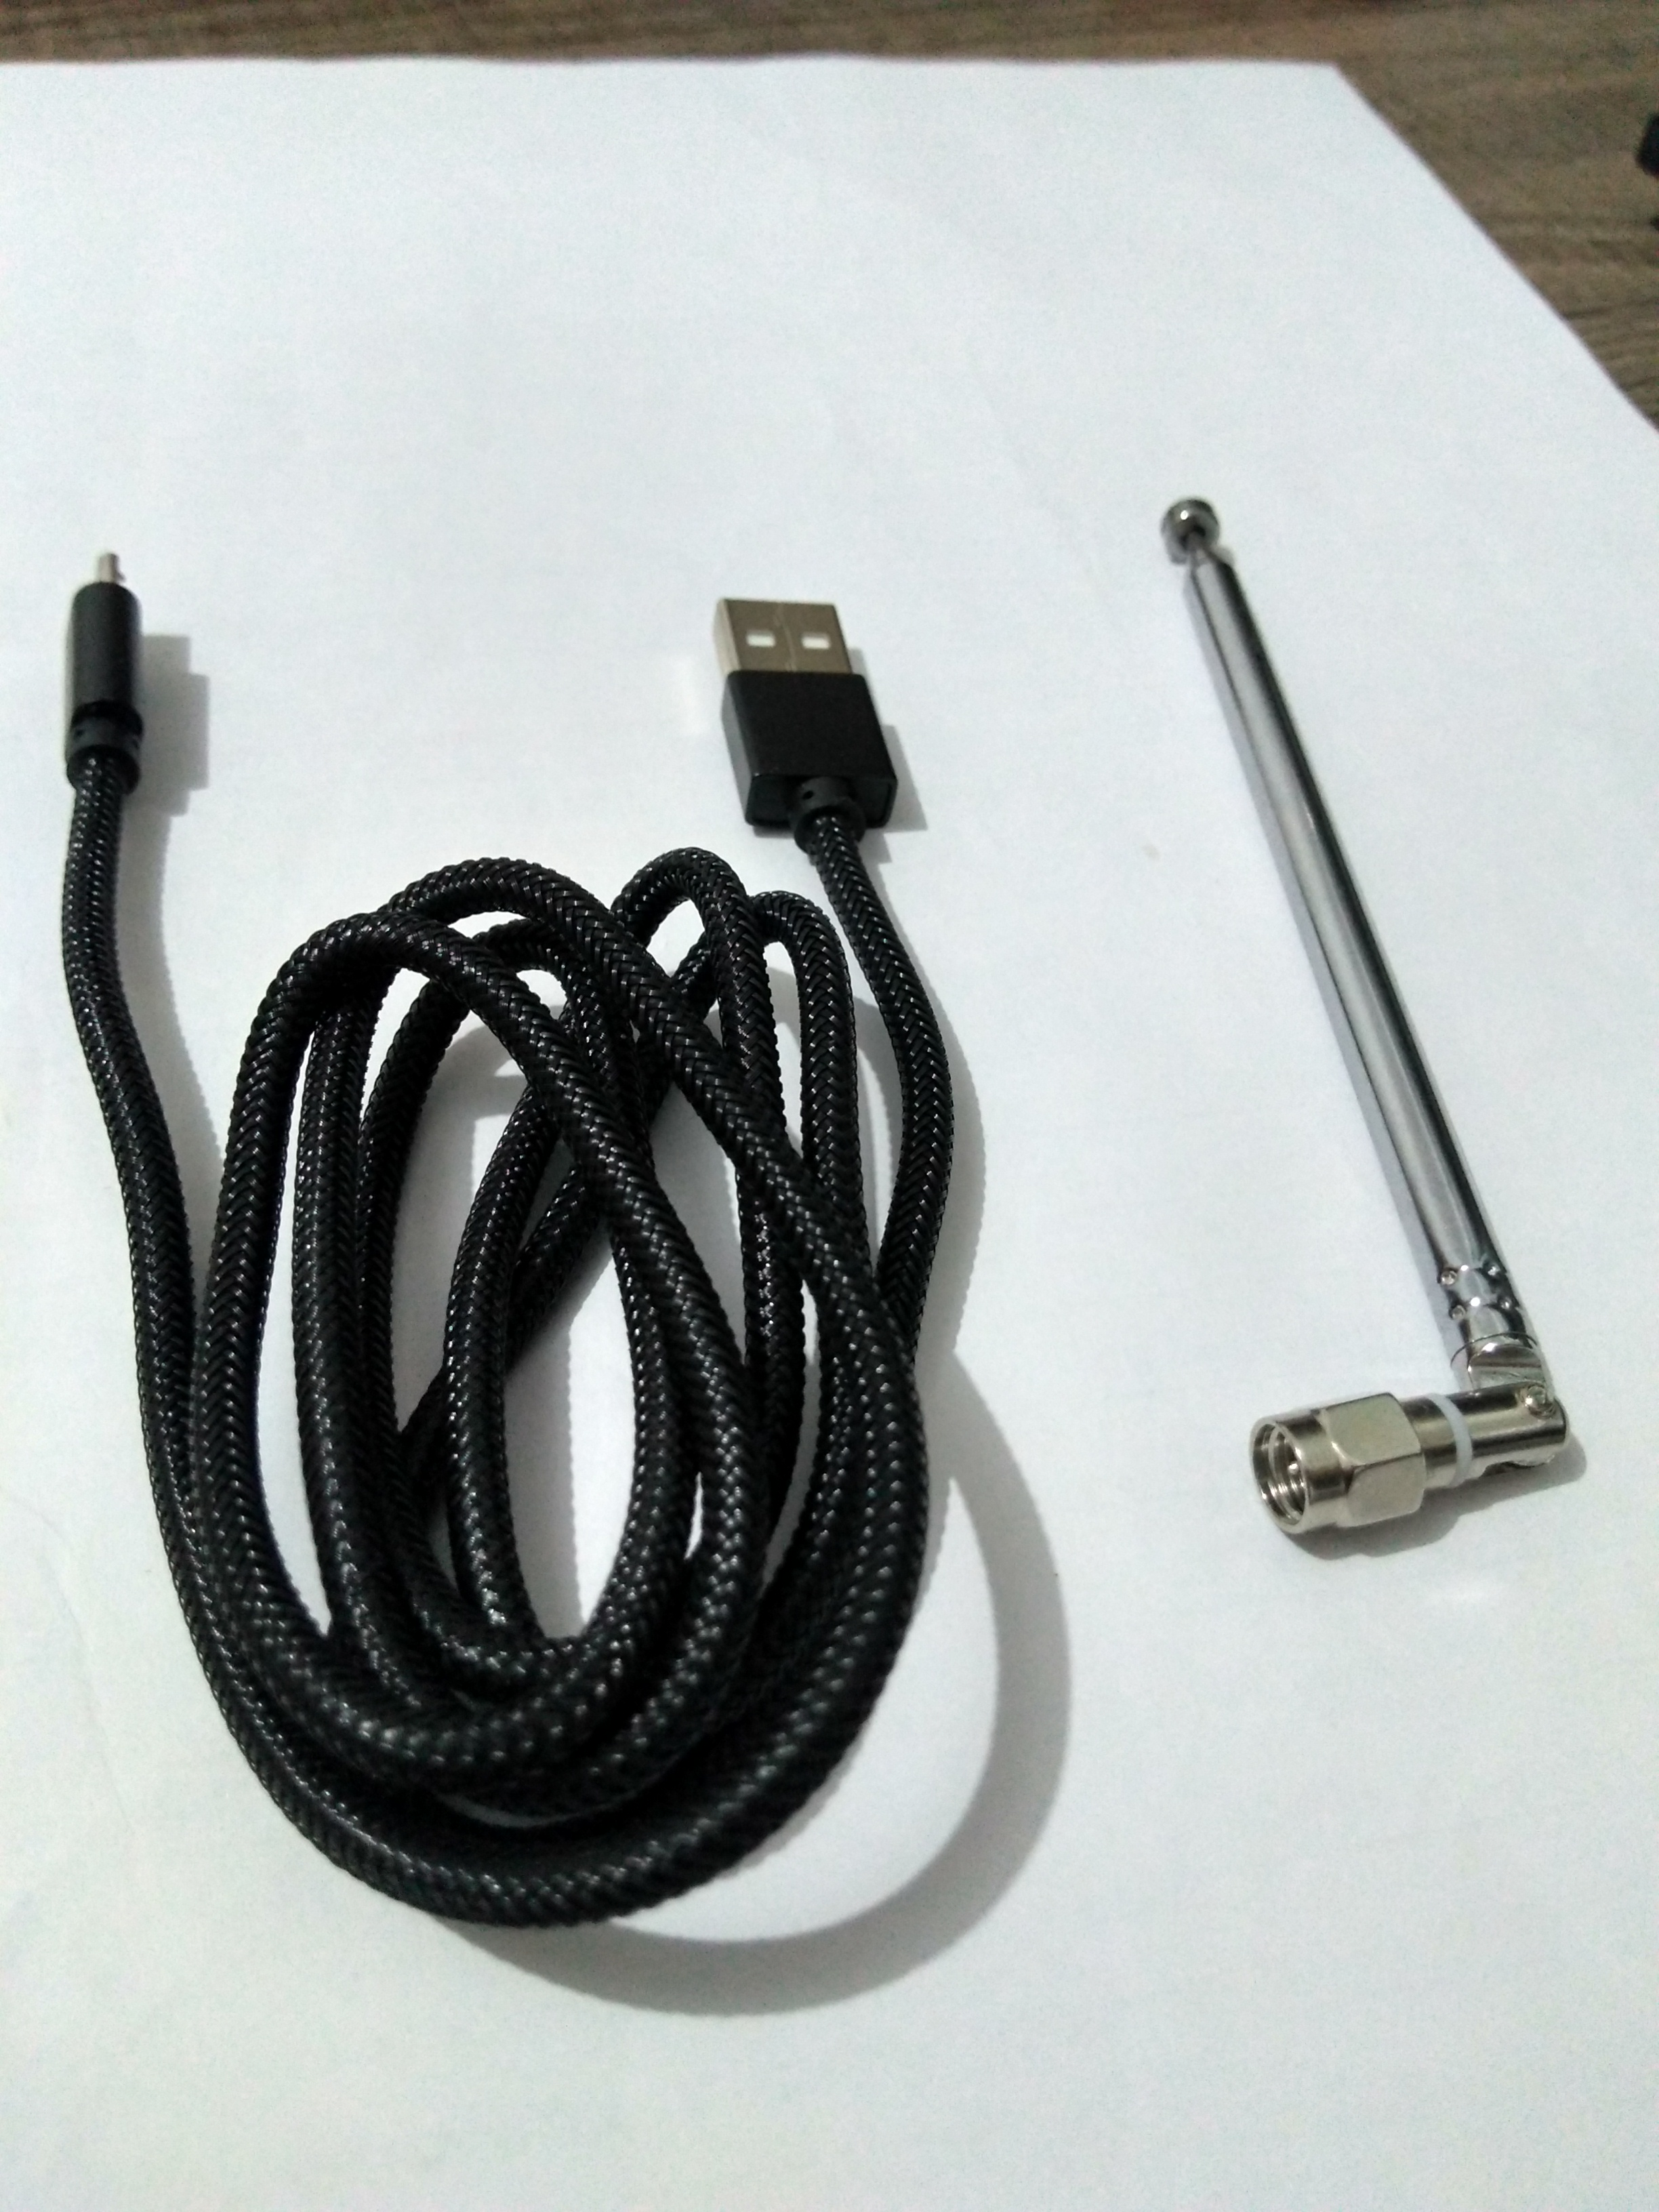
\includegraphics[width=\linewidth]{figures/hackrf/hack_rf_cabo_usb_antena_linear.jpg}
    \caption{Cabo USB e antena telescópica.}
    \label{fig:hack_rf_cabo_usb_antena_linear}
  \end{subfigure}
  \hspace{0.5cm}
  \begin{subfigure}[b]{0.45\linewidth}
    \centering
    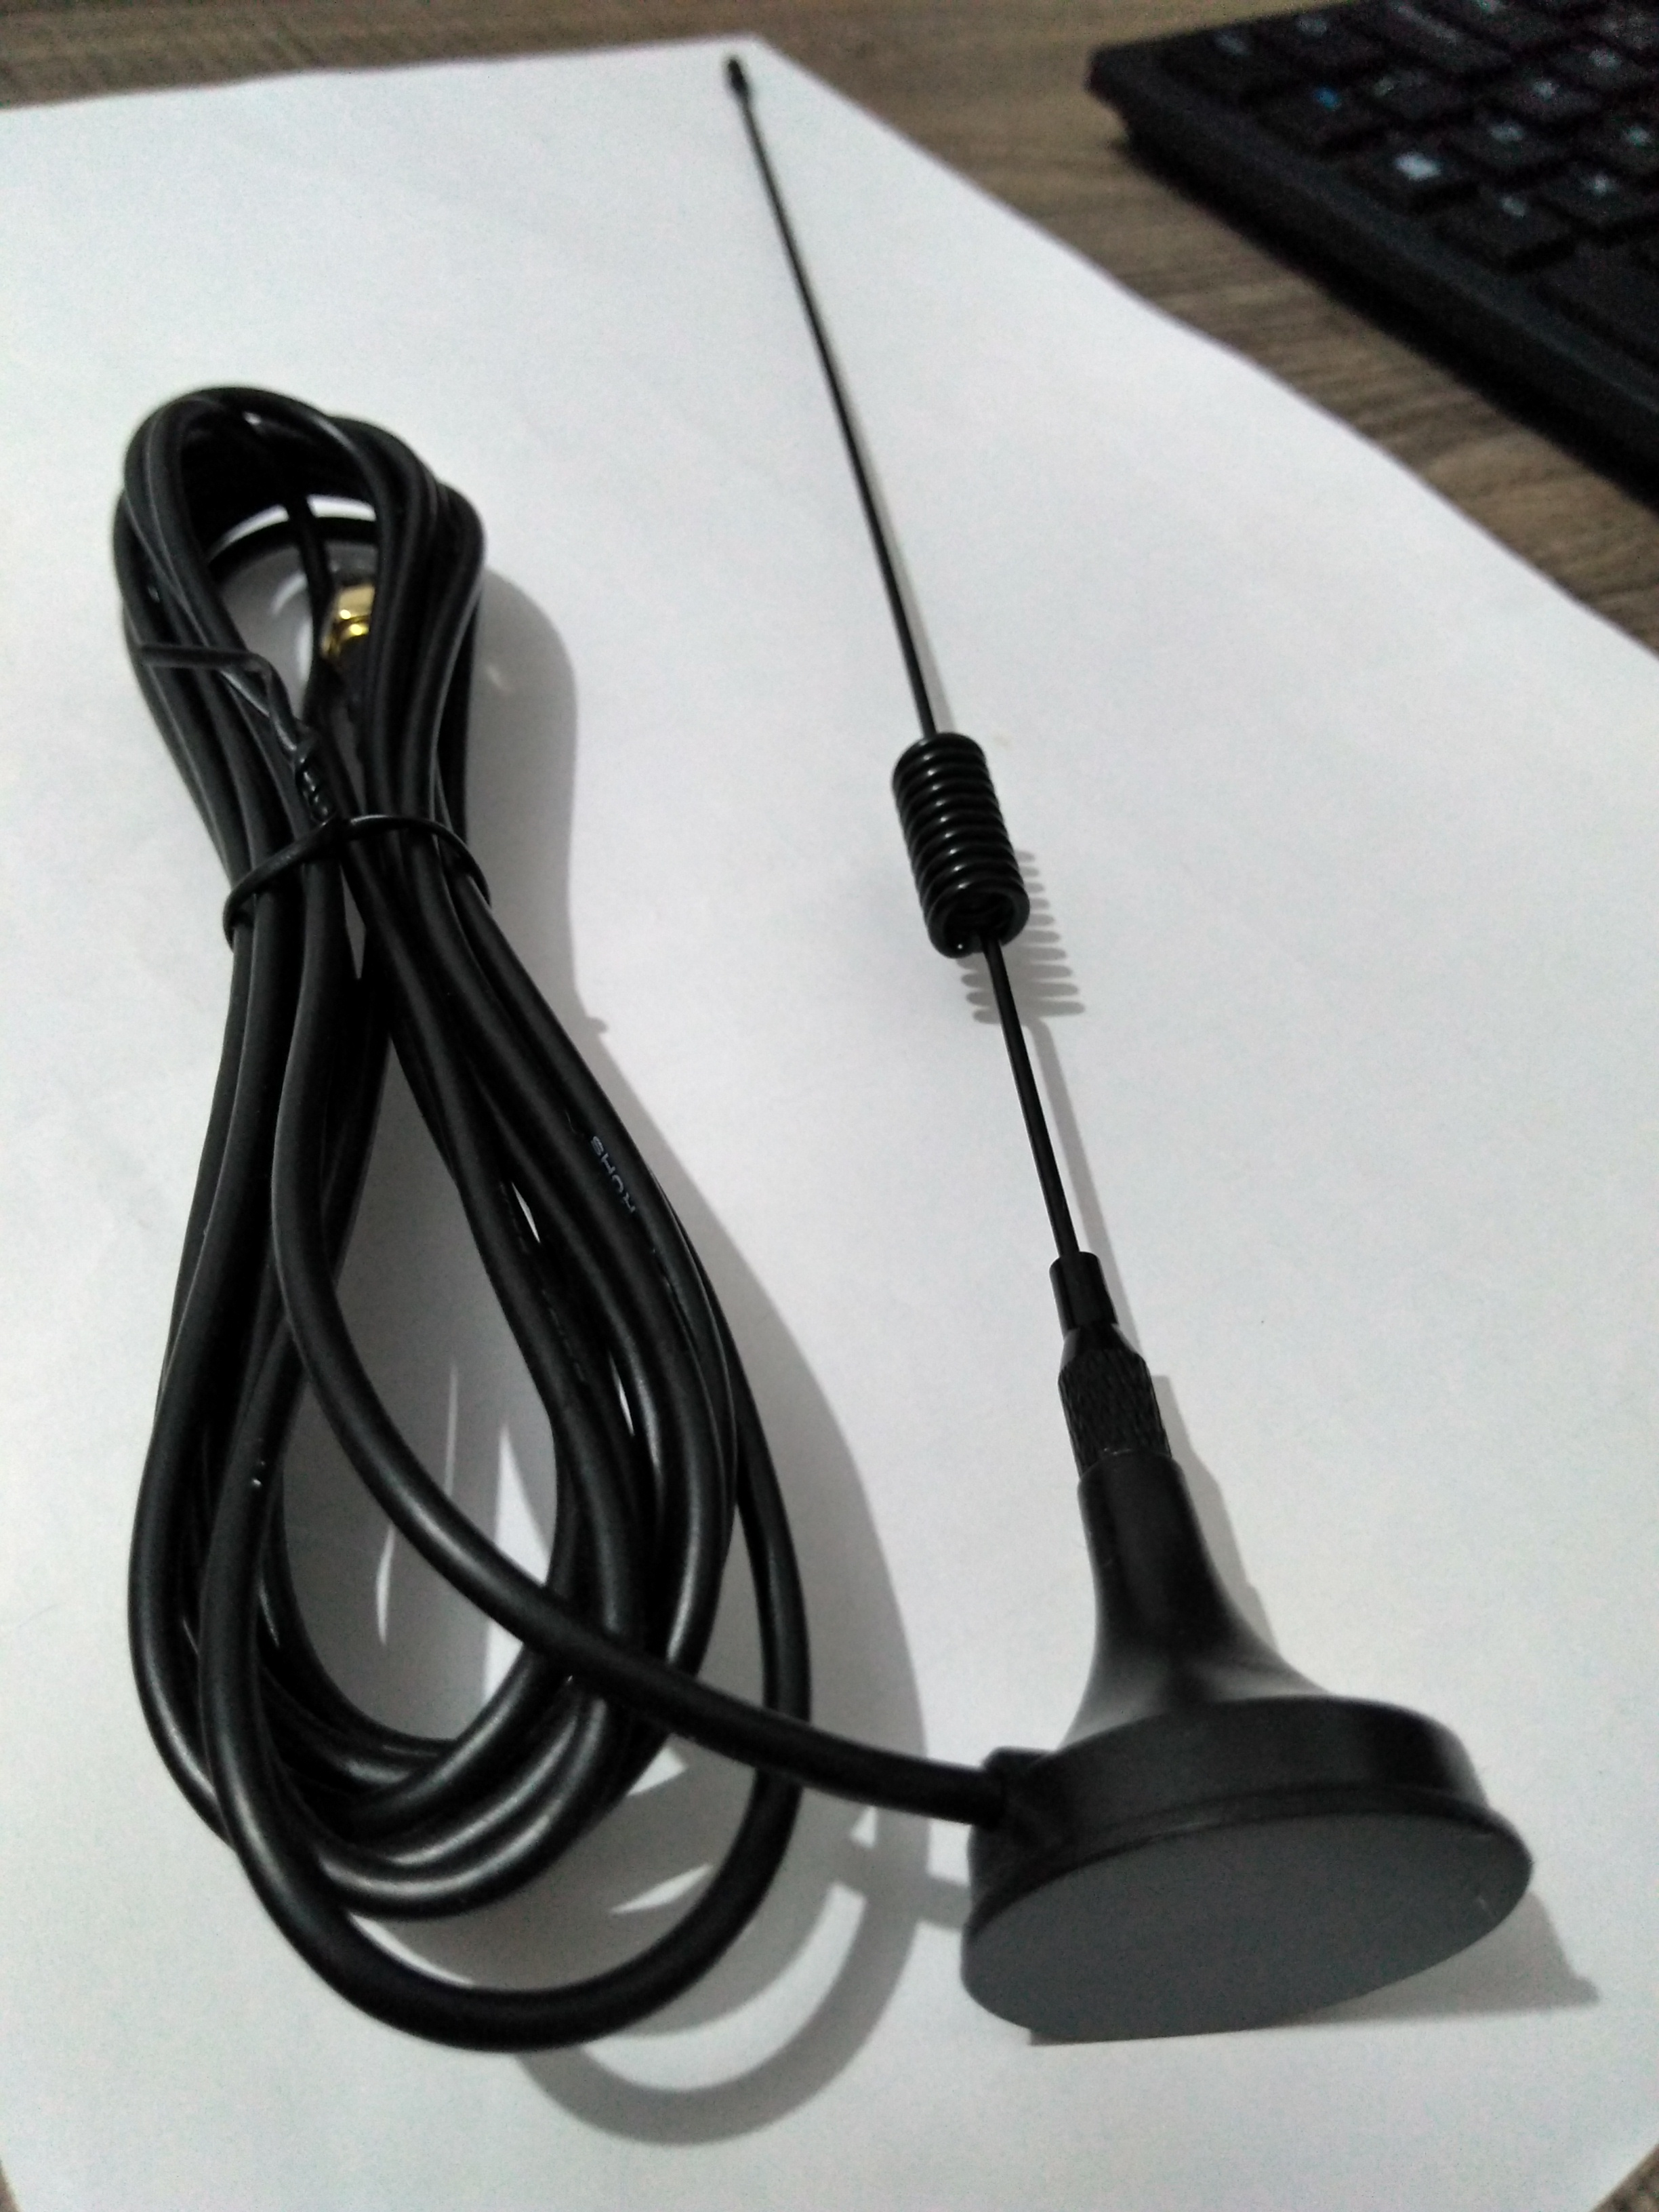
\includegraphics[width=\linewidth]{figures/hackrf/hack_rf_antena_helicoidal.jpg}
    \caption{Antena Omnidirecional.}
    \label{fig:hack_rf_antena_helicoidal}
  \end{subfigure}
  \quad
  \begin{subfigure}[b]{0.45\linewidth}
    \centering
    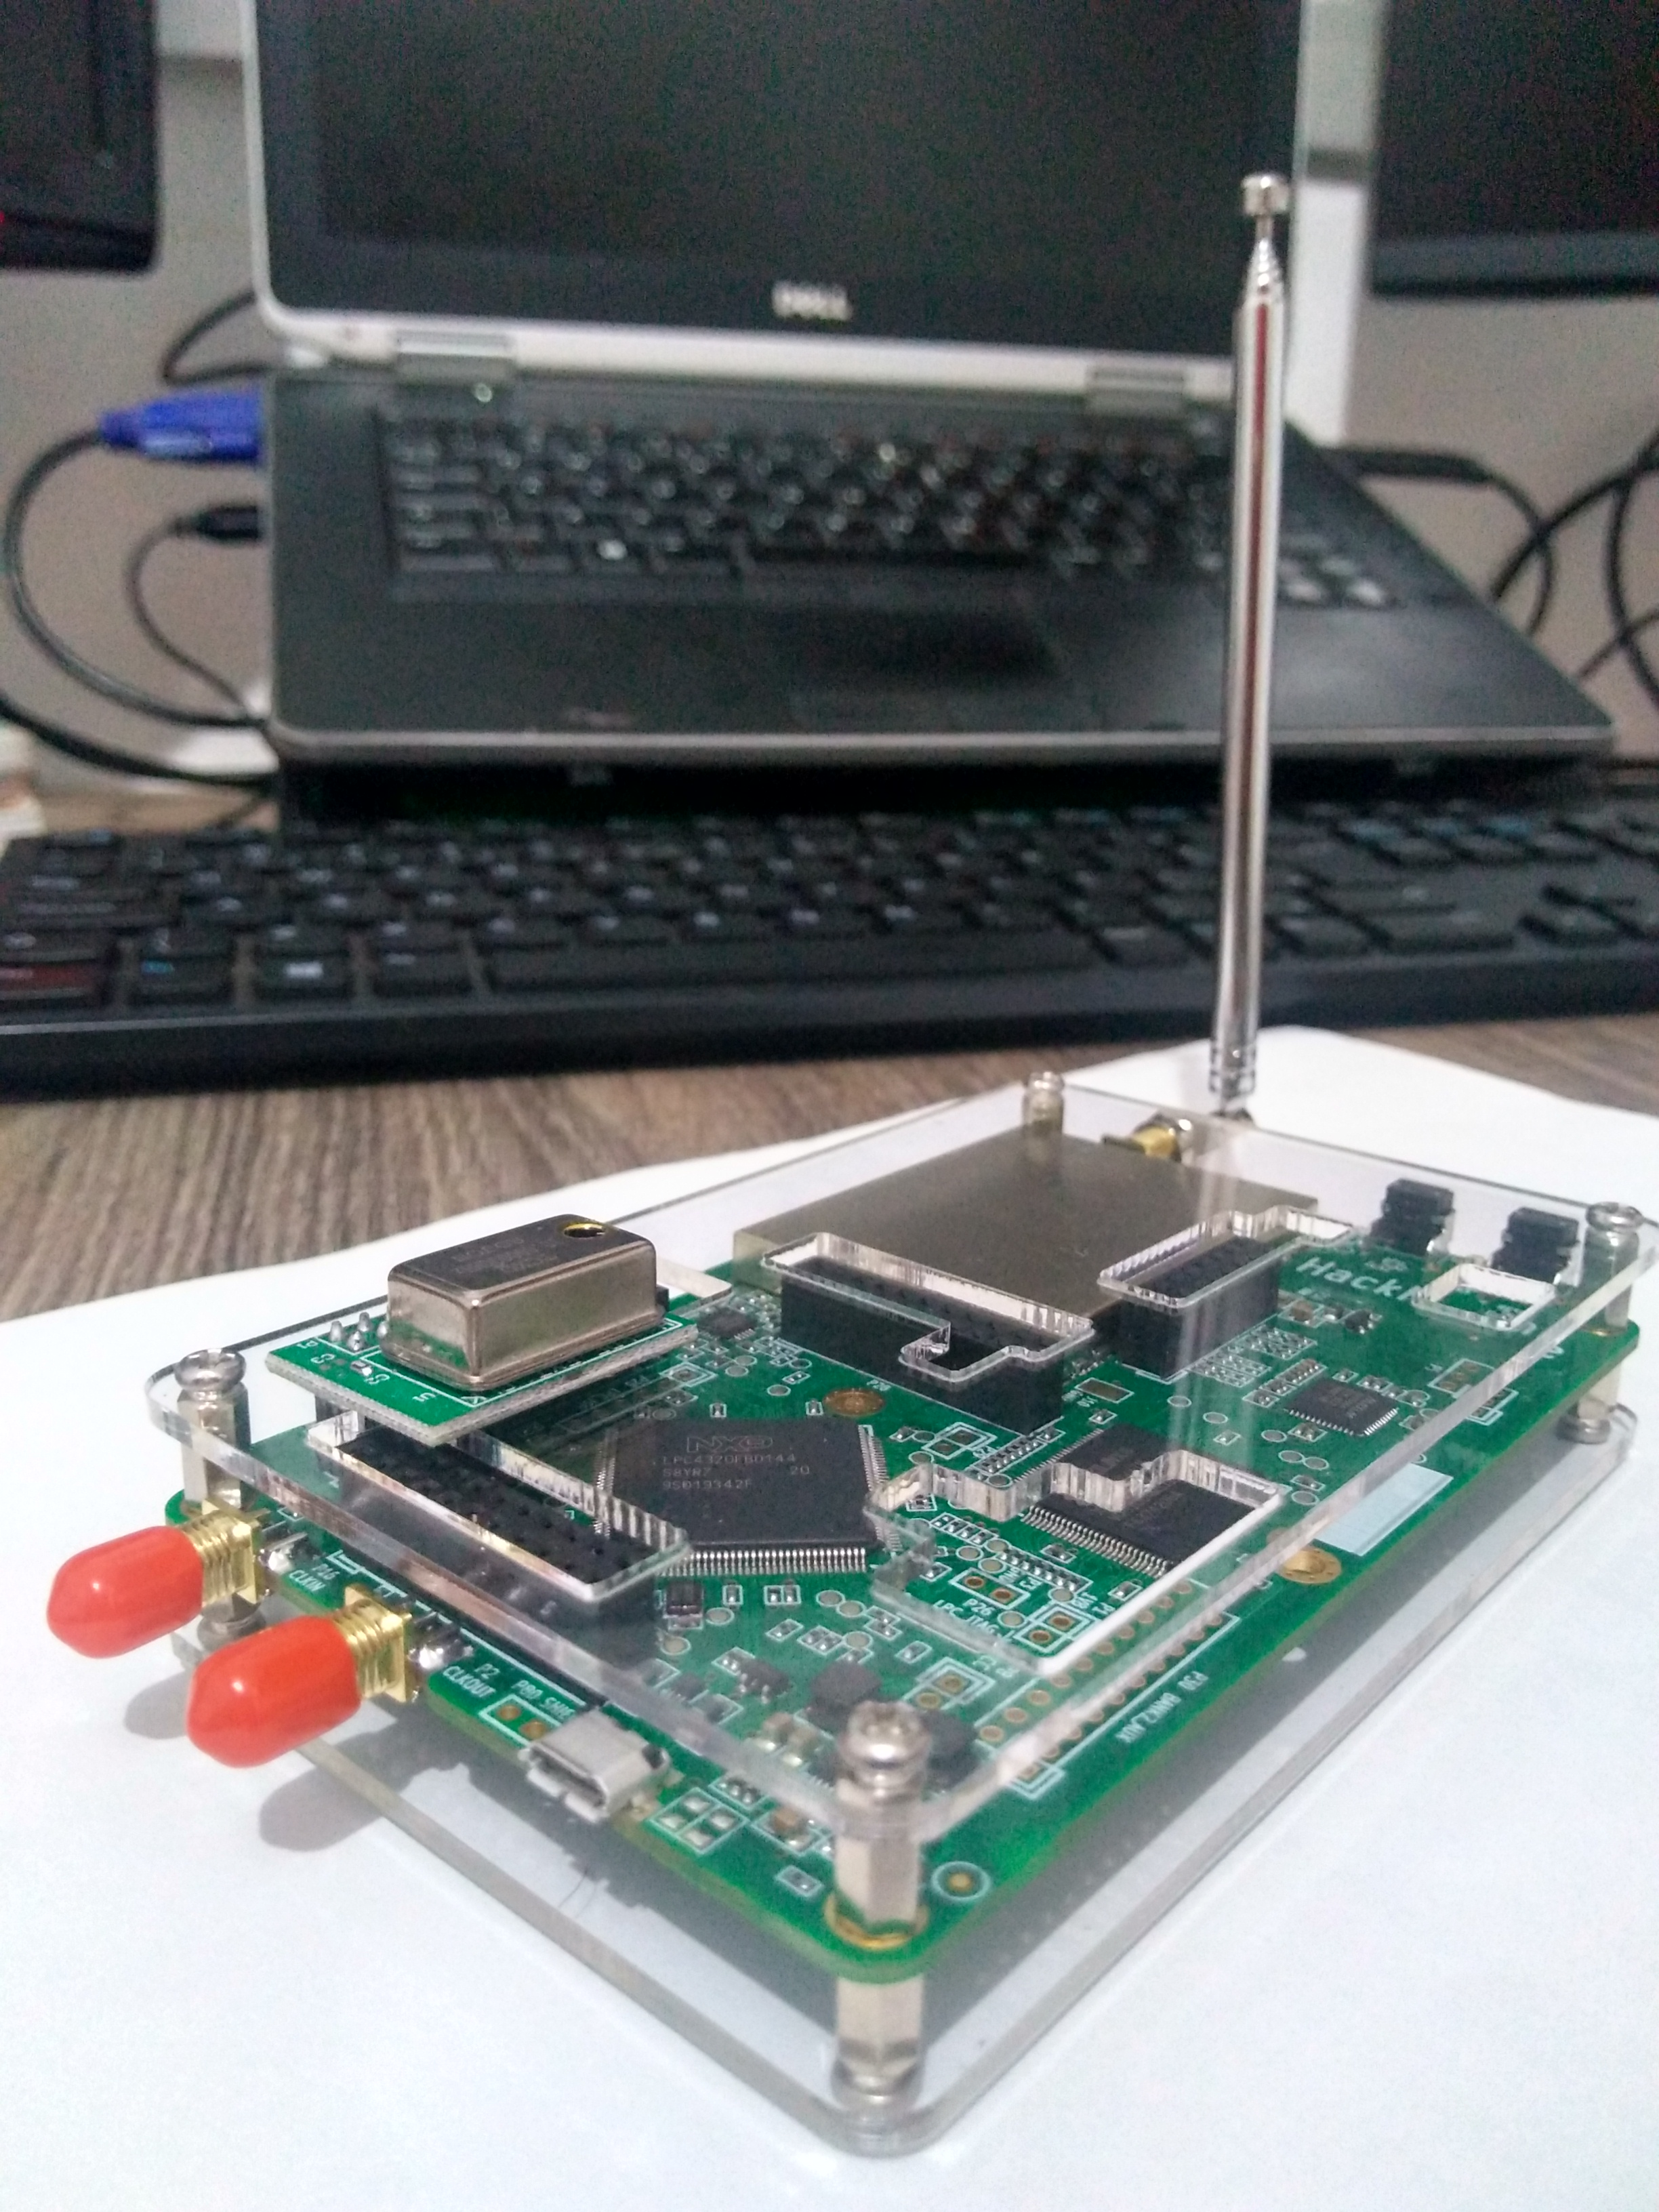
\includegraphics[width=\linewidth]{figures/hackrf/hack_rf.jpg}
    \caption{HackRF com TCXO.}
    \label{fig:hack_rf}
  \end{subfigure}
  \hspace{0.5cm}
  \begin{subfigure}[b]{0.45\linewidth}
    \centering
    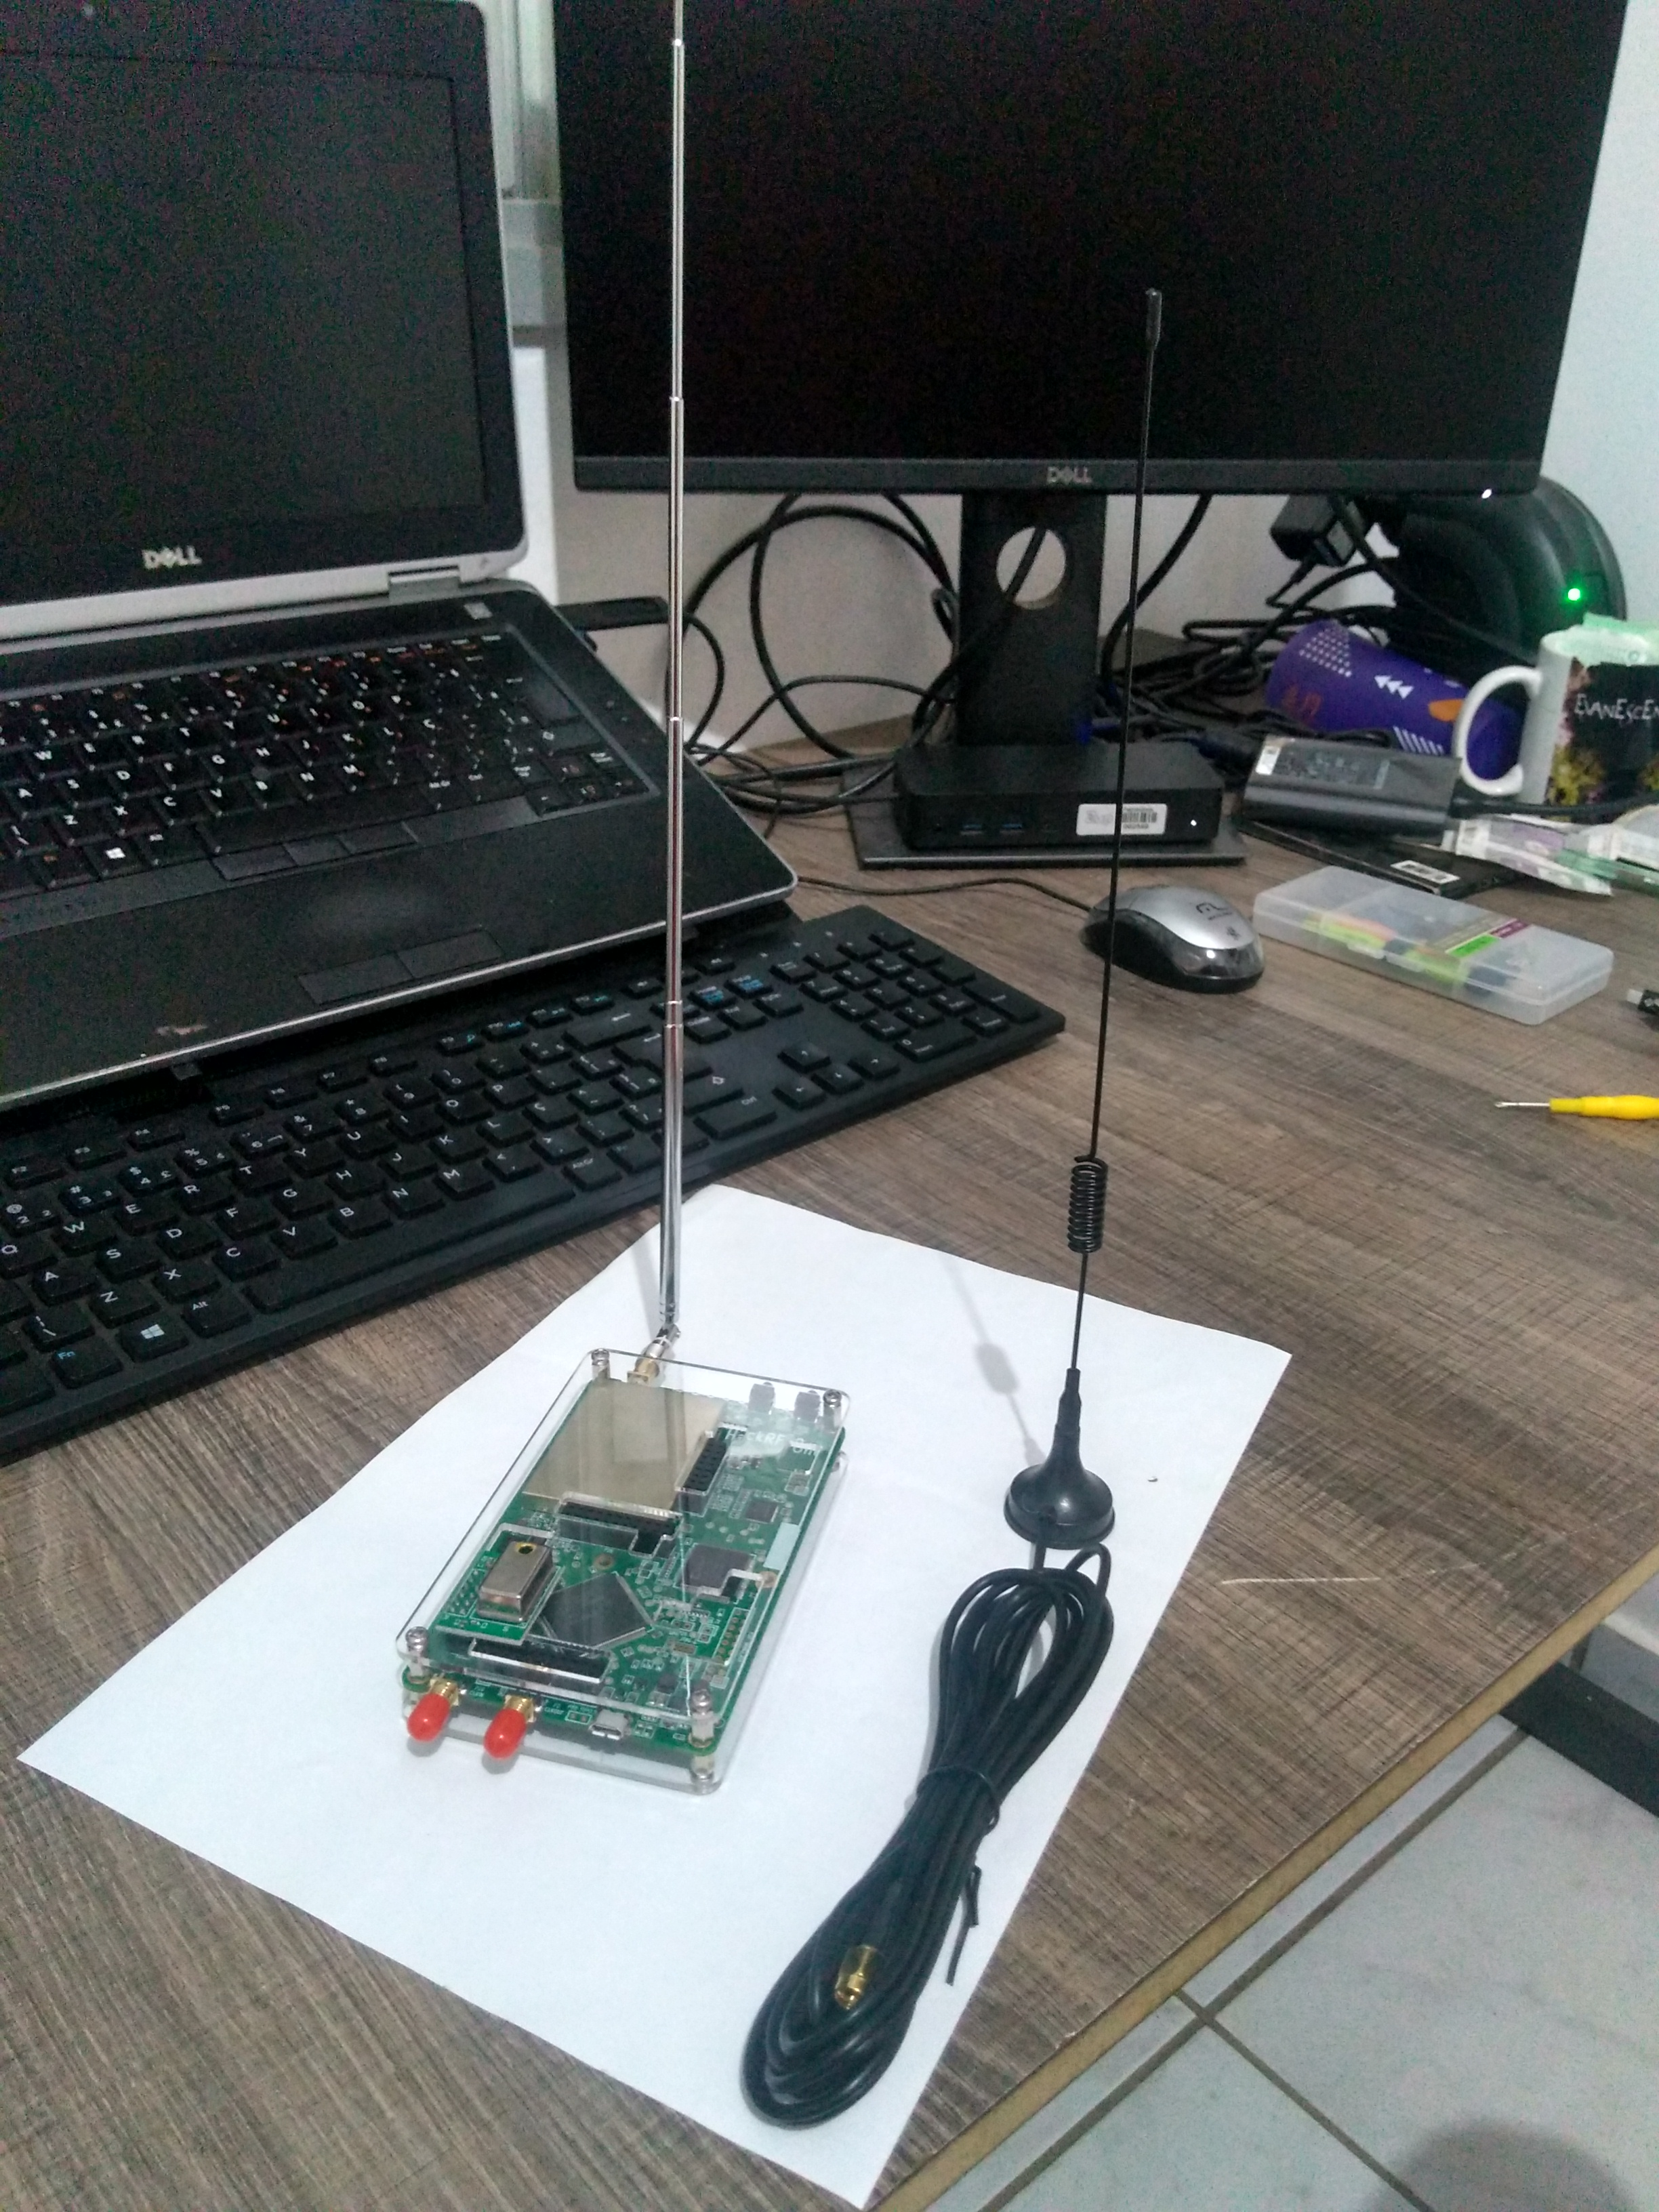
\includegraphics[width=\linewidth]{figures/hackrf/hack_rf_kit.jpg}
    \caption{Kit completo.}
    \label{fig:hack_rf_kit}
  \end{subfigure}
  \caption{\textit{Kit} de desenvolvimento de aplicações de rádio definido por software.}
  \label{fig:hack_rf_hdk}
\end{figure}

\chapter{Software}

O conceito e as boas práticas relacionadas ao desenvolvimento de \textit{software} evoluiu bastante desde os primórdios da computação e algo que sempre esteve
em pauta é o problema de incompatibilidade de ambientes de desenvolvimento, o que acabou dando origem ao jargão: “na minha máquina funciona”.
Configurar o ambiente de desenvolvimento e depois ter incompatibilidade de versão de alguma biblioteca ou então não ter a facilidade de replicar o ambiente
que foi utilizado durante o desenvolvimento é um grande problema enfrentado por engenheiros e/ou programadores \cite{meng2017facilitating}, principalmente os que estão em início de carreira.
Nesta parte deste trabalho será demonstrada a criação de um ambiente para desenvolvimento de aplicações de rádio definido por \textit{software} utilizando
o \textbf{GNURadio} instalado em um \textit{container} \textbf{Docker}.
Os conceitos de \textit{container}'s e do \textit{Docker} com certeza já são amplamente abordados na atualidade e então, apenas alguns pontos relacionados ao tema
serão tratados aqui.

\section*{GNURadio}

O GNURadio é um SDK (\textit{software development kit}) de um projeto \textit{OpenSource} criado com o intuito de auxiliar no desenvolvimento de aplicações de
rádio definido por \textit{software} inicialmente publicado no ano de 2001 como um pacote oficial GNU. Este \textit{software} pode ser utilizado tanto por \textit{hobbystas}, como
também em meio acadêmico ou para suprir necessidades do mercado no que tange comunicações sem fio ou qualquer tipo de sistema de rádio digital do mundo real.
O GNURadio está sob uma licença pública geral — GNU GPLv3 — da \textit{Free Software Foundation} (FSF).

Por ser um projeto de \textit{software} agnóstico ao \textit{hardware} das plataformas de desenvolvimento, o GNURadio é idealizado
para trabalhar apenas com dados digitalizados e a partir disso executar um processamento digital de sinais (DSP — \textit{Digital Signal Processing})
definido por aplicações escritas para receber ou enviar dados de sistemas de \textit{streaming} digital programaticamente, utilizando a linguagem de programação
Python — que é considerado mais fácil — ou C++ — para escrita de códigos de desempenho crítico — além de também ser possível através de uma interface gráfica de
usuário (\textbf{GNURadio Companion} — GRC) por diagramas de blocos.

\newpage
\section*{Docker}

O \textit{Docker} é uma unidade padrão de \textit{software} da empresa \textit{Docker} Inc., que fornece uma camada de abstração e automação em containers, ou seja, grupos isolados de
processos do \textit{kernel} Linux sendo executados e compartilhando os recursos de um mesmo \textit{host}. Um bom entendimento sobre os \textit{namespaces} do  sistema operacional
Linux (\textbf{mnt}, \textbf{pid}, \textbf{net}, \textbf{ipc}, \textbf{uts}, \textbf{user} e \textbf{cgroups}) pode ajudar na compreensão de quais soluções os
\textit{containers} podem oferecer.

Um questionamento bastante pertinente que pode vir à tona neste momento é: Seria mesmo necessário utilizar \textit{container}'s para criação
do ambiente de desenvolvimento, sendo que o próprio GNURadio já é distribuído oficialmente em pacotes compatíveis com os principais sistemas
operacionais encontrados no mercado? Com o decorrer do próximo capítulo o porquê se torna mais claro e por agora a ideia principal é de
que quanto mais isolado possível for o ambiente de desenvolvimento, mais fácil será para testar hipóteses, criar diferentes soluções e tornar
possível que elas sejam reproduzidas com facilidade independentemente se o código que foi desenvolvido em um sistema \textit{host} está sendo executado em outro.

Muitas ferramentas que podem ser úteis para engenheiros e desenvolvedores de \textit{software} para gerenciar ou solucionar problemas podem não estar
incluídas no sistema \textit{host} de suas máquinas por padrão e a melhor maneira de adicionar ferramentas a um \textit{host} seria
incluindo-as em um \textit{container} possibilitando que o \textit{host} seja o mais "enxuto" possível.

Os \textit{container}'s são projetados para manter suas próprias visualizações contidas de \textit{namespaces} e têm acesso limitado aos \textit{hosts} nos quais
são executados. Por padrão, os \textit{container}'s têm uma tabela de processos, interfaces de rede, sistemas de arquivos e recursos IPC
(\textit{Inter-Process Communication}) separados do \textit{host}.
Muitos recursos de segurança, como por exemplo o SELinux (\textit{Security-Enhanced Linux}), são colocados em \textit{container}'s para controlar o acesso ao sistema \textit{host} e outros
\textit{container}'s. Embora os \textit{container}'s possam usar recursos do \textit{host}, os comandos executados a partir de um \textit{container} têm uma capacidade muito
limitada de interagir diretamente com o \textit{host}.

Alguns \textit{container}'s, entretanto, têm como objetivo acessar, monitorar e, possivelmente, alterar recursos no sistema \textit{host}
diretamente \cite{RHEL-container:2020}. Eles são chamados de \textit{container}'s super privilegiados (SPC - \textit{Super Privileged Container}). Um desenvolvedor
pode \textit{subir} um SPC em um \textit{host}, solucionar um problema e removê-lo quando não for mais necessário para liberar recursos.

No próximo capítulo é mostrado como utilizar dos \textit{container}'s super privilegiados para a criação do ambiente de
desenvolvimento de aplicações de \textit{software} e como os recursos de um sistema \textit{host} são acessados a partir desse SPC.

\section*{Criação do ambiente de desenvolvimento}

Primeiramente é necessário ter a CLI (\textit{Command Line Interface}) do \textbf{docker engine} instalada (na máquina \textit{host}) e tal procedimento de
instalação se torna extremamente simples bastando seguir o passo-a-passo fornecido pela \href{https://docs.docker.com/engine/install/}{documentação oficial}
do \textit{Docker} \cite{Docker:2020}.
Esta CLI está disponível para várias distribuições Linux na versão \textit{Server} e também para Windows e Mac na versão \textit{Desktop}. Neste trabalho será
demonstrado o procedimento de instalação do \textbf{docker engine} em uma distribuição Linux, de forma que este procedimento é semelhante para demais distribuições
e arquiteturas.

\subsection*{Instalação do \textit{Docker Engine}}

O \textit{Docker} fornece pacotes prontos (\textbf{.deb} e \textbf{.rpm}) para instalação dessa CLI em distribuições Linux como \textit{CentOS}, \textit{Debian},
\textit{Fedora}, \textit{Raspbian}, \textit{Ubuntu} e derivadas (\textit{LMDE}, \textit{BunsenLabs Linux}, \textit{Kali Linux}, \textit{Kubuntu}, \textit{Lubuntu}
e \textit{Xubuntu}, por exemplo) para arquiteturas \textbf{x86\_64}/\textbf{amd64}, \textbf{ARM} (\textit{Advanced RISC Machine}) e \textbf{ARM64}/\textbf{AARCH64}.
Outra opção de instalação seria utilizando os binários pré-compilados que são fornecidos no site do \textit{Docker} e essa forma
faz bastante sentido quando o sistema operacional utilizado não fizer parte de algum dentre todos os suportados
pelo \textit{Docker}.

Antes de iniciar o procedimento de instalação é necessário verificar se o sistema operacional do \textit{host} utilizado está instalado em uma versão de hardware
de arquitetura 64-bit (\textbf{x86\_64} ou \textbf{amd64}, \textbf{armhf} e \textbf{arm64}/\textbf{aarch64}) e não possui instalações de versões antigas
do \textit{software} (\textbf{docker}, \textbf{docker.io}, ou \textbf{docker-engine}) e, caso hajam, é necessário removê-las. No sistema
operacional Ubuntu basta utilizar o gerenciador de pacotes \textbf{apt}/\textbf{apt-get} para fazê-lo, conforme é exemplificado a seguir:

\begin{adjustbox}{max width=\linewidth}
  \begin{lstlisting}[language=bash]
  $ sudo apt-get remove docker-engine \
    docker docker.io containerd runc
  \end{lstlisting}
\end{adjustbox}

\subsubsection*{Instalação utilizando o repositório ofical}

Utilizar o gerenciador de pacotes presente na distribuição Linux facilita o processo de instalação e remoção de \textit{software} do sistema operacional e esta intalação será feita
utilizando o pacote fornecido no repositório oficial do \textit{Docker}. O primeiro
passo é atualizar a lista de pacotes através do comando \textbf{apt-get update} e instalar algumas dependências que permitem que o gerenciador de pacotes (\textbf{apt}) use um repositório sobre HTTPS.
Os comandos são exemplificados como segue:

\newpage
\begin{adjustbox}{max width=\linewidth}
  \begin{lstlisting}[language=bash]

  $ sudo apt-get update

  $ sudo apt-get install \
    apt-transport-https \
    ca-certificates \
    curl \
    gnupg-agent \
    software-properties-common
  \end{lstlisting}
\end{adjustbox}


Após isso é necessário adicionar a chave GPG (\textit{GNU Privacy Guard}) oficial do\textit{Docker} através do comando:

\begin{adjustbox}{max width=\linewidth}
  \begin{lstlisting}[language=bash]
  $ curl -fsSL https://download.docker.com/linux/ubuntu/gpg \
    | sudo apt-key add -
  \end{lstlisting}
\end{adjustbox}

Para verificar se o sistema já possui a chave com o \textit{fingerprint} \textit{Docker} (no momento em que este texto foi escrito,
era \textbf{9DC8 5822 9FC7 DD38 854A E2D8 8D81 803C 0EBF CD88}), o usuário deve pesquisar os últimos 8 caracteres desse \textit{fingerprint}. Neste caso, basta utilizar o comando:

\begin{adjustbox}{max width=\linewidth}
  \begin{lstlisting}[language=bash]
    $ sudo apt-key fingerprint 0EBFCD88
    \end{lstlisting}
\end{adjustbox}

E o retorno do terminal ficará:

\begin{adjustbox}{max width=\linewidth}
  \begin{lstlisting}[language=bash]
  pub   rsa4096 2017-02-22 [SCEA]
  9DC8 5822 9FC7 DD38 854A  E2D8 8D81 803C 0EBF CD88
  uid  [unknown] Docker Release (CE deb) <docker@docker.com>
  sub   rsa4096 2017-02-22 [S]
\end{lstlisting}
\end{adjustbox}

Feito isso, o próximo passo será configurar que o repositório mais estável ("\textit{stable}") do \textit{Docker} seja indexado ao gerenciador de
pactotes do sistema, o \textbf{apt}:

\begin{adjustbox}{max width=\linewidth}
  \begin{lstlisting}[language=bash]
  $ sudo add-apt-repository \
  "deb [arch=amd64] https://download.docker.com/linux/ubuntu \
  $(lsb_release -cs) \
  stable"
\end{lstlisting}
\end{adjustbox}


Finalmente, as versões mais recentes do \textbf{containerd} e do \textit{Engine} do \textit{Docker} podem ser instaladas após atualizar os índices do
gerenciador de pacotes \textbf{apt}.

\begin{adjustbox}{max width=\linewidth}
  \begin{lstlisting}[language=bash]
  $ sudo apt-get update
  $ sudo apt-get install docker-ce \
    docker-ce-cli containerd.io
\end{lstlisting}
\end{adjustbox}

Para verificar se a instalação foi bem-sucedida, basta executar o comando de testes a seguir que é o "\textit{hello-world}" do \textit{Docker}. Se tudo ocorrer bem,
o terminal responderá com uma saída semelhante ao que é mostrado na Fig. \ref{fig:docker-hello-world}.

\begin{adjustbox}{max width=\linewidth}
  \begin{lstlisting}[language=bash]
  $ sudo docker run hello-world
\end{lstlisting}
\end{adjustbox}

\begin{figure}[!htb]
  \centering
  \caption{Teste de verificação de instalação do \textit{Docker Engine}.}
  \includegraphics[width = \linewidth]{figures/docker-hello-world.png}
  Fonte: Elaborado pelo autor.
  \label{fig:docker-hello-world}
\end{figure}

Neste ponto, o \textit{Docker} encontra-se devidamente instalado no sistema operacional e o usuário pode optar por executar alguns comandos de pós-instalação
para, por exemplo, possibilitar a execução do \textit{Docker} sem a necessidade de ter privilégios de usuário \textit{root}, iniciar o serviço \textit{Docker} na inicialização do
sistema operacional, usar uma \textit{engine} de armazenamento diferente da que vem como padrão de instalação (\textit{overlay2}) dentre outras coisas descritas
na seção de \href{https://docs.docker.com/engine/install/linux-postinstall/}{pós-instalação} da documentação oficial \cite{Docker:post-installation-2020}.

\subsection*{Criação do container}

Com o \textit{Docker} instalado, para inciar o procedimento de criação do \textit{container} do ambiente de desenvolvimento é preciso executar o comando \textbf{xhost +}
para fornecer acesso ao servidor gráfico do \textit{host} a aplicações “externas” ao \textit{host} (também conhecido como sessão \textbf{X} ou a tela do computador),
afinal um dos objetivos é utilizar a interface gráfica do \textit{GNURadio Companion} que estará instalado dentro do \textit{container}.

Agora, executando o seguinte comando será criado um \textit{container} a partir de uma imagem base da distribuição \textit{Ubuntu}. A Fig.
\ref{fig:docker-run-gnuradio} exemplifica o uso do comando e as saídas retornadas pelo terminal e é dentro do \textit{container}
criado que será feita a instalação do GNURadio.

\begin{adjustbox}{max width=\linewidth}
  \begin{lstlisting}[language=bash]
$  docker run -i -t --privileged \
    --ipc=host --net=host --pid=host -e HOST=/host \
    -e DISPLAY=$DISPLAY \
    -e DCONF_PROFILE=/etc/dconf/profile/ \
    -e XDG_DATA_HOME=/config/xdg/data \
    -e XDG_CONFIG_HOME=/config/xdg/config \
    -e XDG_CACHE_HOME=/config/xdg/cache \
    -e XDG_RUNTIME_DIR=/tmp/runtime-root \
    -e DBUS_SESSION_BUS_ADDRESS="$DBUS_SESSION_BUS_ADDRESS" \
    -e DEBIAN_FRONTEND="noninteractive" \
    -e IMAGE=jeffcandido/gnuradio \
    -v /run:/run -v /var/log:/var/log\
    -v /etc/localtime:/etc/localtime -v /:/host \
    -v /etc/dconf/profile/:/etc/dconf/profile/ \
    -v /tmp/runtime-root/:/tmp/runtime-root/ \
    -v /tmp/.X11-unix/:/tmp/.X11-unix \
    -v /dev/usb:/dev/usb \
    -v /dev/snd:/dev/snd \
    -v /home/jefferson/gnuradio:/home/jefferson/gnuradio \
    --name gnuradio \
    ubuntu:20.04
  \end{lstlisting}
\end{adjustbox}


\begin{figure}[!htb]
  \centering
  \caption{Criação do \textit{container} de desenvolvimento a partir de uma imagem Ubuntu.}
  \includegraphics[width = \linewidth, trim = 0.1cm 5cm 12cm 0.1cm, clip = true]{figures/docker-run-gnuradio.png}
  Fonte: Elaborado pelo autor.
  \label{fig:docker-run-gnuradio}
\end{figure}

Para melhorar o entendimento, essa linha vai ser dividida e explicada por partes. O comando \textbf{docker run} primeiro cria uma camada de \textit{container}
gravável sobre a imagem especificada (Ubuntu) e, em seguida, o inicia usando o comando especificado. Ou seja, \textbf{docker run} é equivalente a utilizar
\textbf{docker container create} e depois \textbf{docker container start}. Um \textit{container} interrompido pode ser reiniciado com todas as suas alterações anteriores
intactas usando \textbf{docker start}. Agora, sobre as \textit{flags} passadas:

\begin{itemize}
  \item[$-$] \textbf{i} (\textbf{interactive}): manter o \textbf{STDIN} (\textit{standard input} — fluxo de entrada padrão) aberto, mesmo se não estiver conectado;
  \item[$-$] \textbf{t} (\textbf{tty}): alocar um pseudo-\textbf{TTY} (\textit{TeleTYpewriter} — simplesmente um terminal ao qual o usuário está conectado);
  \item[$-$] \textbf{privileged}: dar privilégios estendidos a este \textit{container} (desativa a separação de segurança entre o \textit{host} e o
        \textit{container}, o que significa que um processo executado como \textit{root} dentro do \textit{container} tem o mesmo acesso ao \textit{host}
        que ele poderia também ter se fosse executado de fora do \textit{container}.);
  \item[$-$] \textbf{e} (\textbf{env}): definir variáveis de ambiente;
  \item[$-$] \textbf{v} (\textbf{volume}): vincular a montagem de um volume dentro do \textit{container};
  \item[$-$] \textbf{name}: o nome que se dará ao \textit{container} criado.
  \item[$-$] As \textit{flags} \textbf{--ipc=host}, \textbf{--net=host} e \textbf{--pid=host} desligam os \textit{namespaces} \textbf{ipc},
        \textbf{net} e \textbf{pid} dentro do \textit{container}. Isso significa que os processos dentro do \textit{container} veem a mesma rede e
        tabela de processos, bem como compartilham quaisquer IPCs \cite{Rusling-IPC:1999} com os processos do \textit{host}.
\end{itemize}

Indo um pouco mais a fundo, tem-se a configuração de algumas variáveis de ambiente e a definição dos pontos de montagem e vinculação de alguns
\textit{volumes} ao \textit{host}. Em tese, estas variáveis de ambiente foram configuradas porque foram observadas algumas necessidades durante o
desenvolvimento deste trabalho, tais quais:

\begin{itemize}
  \item[$-$] \textbf{HOST=/host}: definir uma variável que possa ser usada dentro do \textit{container} para acessar
        arquivos e diretórios a partir da raiz do \textit{filesystem} do \textit{host};
  \item[$-$] \textbf{DISPLAY=\$DISPLAY}: definir uma variável que identifique onde serão exibidos recursos pelo servidor gráfico \textbf{X};
  \item[$-$] \textbf{DCONF\_PROFILE=/etc/dconf/profile/}: definir a variável relacionada a um sistema de armazenamento das
        preferências de usuário \cite{GNOME-dconf-overview:2020};
  \item[$-$] \textbf{XDG\_DATA\_HOME=/config/xdg/data}: definir qual será o único diretório base relativo ao qual os arquivos
        de dados específicos do usuário devem ser gravados \cite{freedesktop-XDG:2020};
  \item[$-$] \textbf{XDG\_CONFIG\_HOME=/config/xdg/config}: definir qual será o único diretório base relativo ao qual os arquivos
        de configuração específicos do usuário devem ser gravados \cite{freedesktop-XDG:2020};
  \item[$-$] \textbf{XDG\_CACHE\_HOME=/config/xdg/cache}: definir qual será o único diretório base relativo ao qual os dados não
        essenciais específicos do usuário (em cache) devem ser gravados \cite{freedesktop-XDG:2020};
  \item[$-$] \textbf{XDG\_RUNTIME\_DIR=/tmp/runtime-root}: definir qual será o único diretório base relativo ao qual os arquivos de
        tempo de execução específicos do usuário e outros objetos de arquivo devem ser colocados;
  \item[$-$] \textbf{DBUS\_SESSION\_BUS\_ADDRESS=}

        \textbf{"\$DBUS\_SESSION\_BUS\_ADDRESS"}: possibilitar a inicialização de uma sessão de barramento usando o utilitário D-Bus \cite{freedesktop-DBUS:2020};
  \item[$-$] \textbf{DEBIAN\_FRONTEND="noninteractive"}: definir variável para silenciar os \textit{prompt}'s de configuração do \textit{container} \cite{Debian:non-interactive};
  \item[$-$] \textbf{IMAGE=jeffcandido/gnuradio}: definir a variável para identificar o nome da imagem.
\end{itemize}

Com relação aos \textit{volumes} que foram montados, seguem suas definições:

\begin{itemize}
  \item[$-$] \textbf{/run}:\textbf{/run}: montar o diretório \textbf{/run} do host no diretório \textbf{/run} dentro do \textit{container}. Isso permite que os processos dentro do
        \textit{container} falem com o serviço \textbf{dbus} do \textit{host} e falem diretamente com o serviço \textbf{systemd};

  \item[$-$] \textbf{/var/log}:\textbf{/var/log}: permitir que comandos sejam executados dentro do \textit{container} para ler e gravar arquivos de log no diretório
        \textbf{/var/log} do \textit{host};

  \item[$-$] \textbf{/etc/localtime}:\textbf{/etc/localtime}: fazer com que o fuso horário do sistema \textit{host} seja usado
        também no \textit{container};

  \item[$-$] \textbf{/}:\textbf{/host}: montar a raiz da árvore de diretórios do \textit{host} (mais conhecida como \textbf{/}) no  ponto
        de montagem \textbf{/host} para permitir que processos dentro do \textit{container} consigam modificar facilmente o conteúdo no \textit{host};

  \item[$-$] \textbf{/etc/dconf/profile/}:\textbf{/etc/dconf/profile/}: vincular o sistema de armazenamento de preferências do usuário ao mesmo do \textit{host} \cite{RHEL-dconf-profile:2020};

  \item[$-$] \textbf{/tmp/runtime-root/}:\textbf{/tmp/runtime-root/}: montar e vincular o diretório base relativo aos arquivos de
        tempo de execução específicos do usuário;

  \item[$-$] \textbf{/tmp/.X11-unix/}:\textbf{/tmp/.X11-unix/}: montar um volume para o \textit{unix socket} X11 (servidor gráfico);

  \item[$-$] \textbf{/dev/usb}:\textbf{/dev/usb}: vincular o volume que possibilita a utilização de recursos da porta USB do \textit{host};

  \item[$-$] \textbf{/dev/snd}:\textbf{/dev/snd}: vincular o volume que possibilita a utilização de recursos de áudio do \textit{host};

  \item[$-$] \textbf{/home/jefferson/gnuradio}:\textbf{/home/jefferson/gnuradio}: montar um diretório que será utilizado no desenvolvimento
        deste trabalho e que poderá ser acessado tanto pelo \textit{host} como pelo \textit{container}.
\end{itemize}

Resumindo, foi utilizada uma linha de comando para criar um \textit{container}, o qual foi nomeado \textbf{gnuradio}, a partir de uma imagem base (Ubuntu) com
privilégios para acessar recursos da máquina (o \textit{host}), onde mais precisamente será possível utilizar os recursos de áudio, da porta USB e da
interface visual com uma vinculação de volumes montados no \textit{container} a partir da máquina \textit{host}.

Algo importante a se notar na Fig. \ref{fig:docker-run-gnuradio} é que depois da criação do \textit{container} o terminal “mudou” do usuário \textbf{jefferson} para \textbf{root}
e manteve o \textit{hostname}. Isso ocorre porque a partir desse momento o que aparece na tela é o terminal visto de "dentro"
do \textbf{container}, ou seja, com o usuário \textbf{root} em um \textit{container} que está enxergando o mesmo \textit{namespace} \textbf{net} que o
sistema \textit{host}.

Em outro terminal é possível obter mais informações como, por exemplo, quais \textit{container}'s estão sendo executados no momento ou inspecionar algum
\textit{container} específico em busca de maiores detalhes, como é mostrado na Fig. \ref{fig:docker-inspect}.

\begin{figure}[!htb]
  \centering
  \caption{Detalhamento de informações sobre \textit{container}’s \textit{Docker}.}
  \includegraphics[width = \linewidth, trim= 0.1cm 0.1cm 20cm 0.1cm, clip=true]{figures/docker-inspect.png}
  Fonte: Elaborado pelo autor.
  \label{fig:docker-inspect}
\end{figure}

\newpage
\subsection*{Instalação do GNURadio}

Até o momento apenas foi feito o provisionamento de um \textit{container} \textit{Docker} executando uma imagem Ubuntu e então o GNURadio será instalado utilizando
o gerenciador de pacotes \textbf{apt} disponível na distribuição Ubuntu deste \textit{container}. É recomendável atualizar a lista dos repositórios e verificar
as depedências para esta instalação bastando executar os seguintes comandos no terminal do \textit{container} criado:

\begin{adjustbox}{max width=\linewidth}
  \begin{lstlisting}[language=bash]
  $ apt-get update && apt-get upgrade
  $ apt-get install gir1.2-gtk-3.0 libx11-dev
  $ apt-get install gnuradio
\end{lstlisting}
\end{adjustbox}

A partir desse ponto, o GNURadio estará instalado no \textit{container} \textit{Docker} e é possível verificar a versão, o local de instalação e os
componentes já habilitados através dos seguintes comandos que foram exemplificados na Fig. \ref{fig:gnuradio-config-info}:

\begin{adjustbox}{max width=\linewidth}
  \begin{lstlisting}[language=bash]
  $ gnuradio-config-info --version
  $ gnuradio-config-info --prefix
  $ gnuradio-config-info --enabled-components
\end{lstlisting}
\end{adjustbox}

\begin{figure}[!htb]
  \centering
  \caption{Conferência de versão, \textit{path} e componentes habilitados do GNURadio.}
  \includegraphics[width = \linewidth]{figures/gnuradio-config-info.png}
  Fonte: Elaborado pelo autor.
  \label{fig:gnuradio-config-info}
\end{figure}

Conforme ilustrado na Fig. \ref{fig:gnuradio-companion}, após todos os procedimentos descritos neste capítulo, o GNURadio na versão \textbf{3.8.1.0} estará
disponível para o desenvolvimento de aplicações de rádio definido por \textit{software} e de processamento digital de sinais utilizando as bibliotecas
que foram instaladas no \textit{container} ou utilizando a GUI — \textit{Graphical User Interface}, interface gráfica de usuário —
através do comando \textbf{gnuradio-companion} (GRC).

\begin{figure}[!htb]
  \centering
  \caption{\textit{GUI} do \textit{GNURadio Companion}.}
  \includegraphics[width = \linewidth]{figures/gnuradio-companion.png}
  Fonte: Elaborado pelo autor.
  \label{fig:gnuradio-companion}
\end{figure}

\subsection*{Criação da imagem \textit{Docker}}

O \textit{container} criado na seção anterior pode ser disponibilizado para outros desenvolvedores por meio da criação de uma imagem
base. A imagem base deve receber uma \textit{tag}, que normalmente está ligada à sua versão e, por fim, esta imagem pode ser
"empurrada" para um repositório de imagens \textit{Docker}. Neste caso, foi utilizado o \textit{DockerHub} que é um repositório
de imagens \textit{Docker} público e hospedado e fornecido pela própria empresa \textit{Docker} Inc. Qualquer empresa pode hospedar, manter
e disponibilizar um repositório de imagens \textit{Docker} por meio da implantação de um \textit{Docker Registry} próprio.

Na Fig. \ref{fig:docker-gnuradio_base_image}, ao executar o comando \textbf{docker images} apenas a imagem \textbf{ubuntu}
foi listada, pois ainda não foi criada uma imagem do container \textbf{gnuradio}, o qual pode ser conferido com o comando
\textbf{docker ps -a}. Utilizando o commando \textbf{docker commit} referenciando para o container \textbf{gnuradio}, uma imagem
\textit{Docker} é criada localmente, onde as \textit{flags} utilizadas, \textbf{-a} e \textbf{-m}, são uma descrição
sobre o autor e uma breve mensagem sobre a imagem criada, respectivamente.

\begin{figure}[!htb]
  \centering
  \caption{Fazendo o \textit{commit} da imagem base GNURadio.}
  \includegraphics[width = \linewidth, trim= 0.1cm 25cm 0.1cm 0.1cm, clip=true]{figures/docker-gnuradio_base_image.png}
  Fonte: Elaborado pelo autor.
  \label{fig:docker-gnuradio_base_image}
\end{figure}

Após o \textit{commit} da imagem, ao executar o comando \textbf{docker images} novamente, observa-se que a imagem foi criada com
um \textbf{IMAGE ID} igual a \textbf{1c66799cf780} faltando apenas que seja associada a um repositório e que tenha uma \textit{tag} de versionamento.
Como exemplo foi criada a \textit{tag} para a imagem e associada a um repositório público através do comando \textbf{docker tag 1c66799cf780 jeffcandido/gnuradio}.
Ao executar \textbf{docker images} novamente, a imagem do \textit{container} contendo a instalação do GNURadio na versão 3.8.1.0
está pronta para ser levada ao repositório de imagens \textit{Docker} e se tornar acessível a outros desenvolvedores. Para
fazer esse procedimento, foi necessário criar uma conta (gratuita) no \textit{DockerHub} e realizar o \textit{login} via linha de comando e finalmente
executar o \textit{push} da imagem para levá-la até o repositório remoto, como é demonstrado nos passos executados na Fig. \ref{fig:docker-push_image}.

\begin{figure}[!htb]
  \centering
  \caption{Submetendo a imagem base ao repositório remoto.}
  \includegraphics[width = \linewidth]{figures/docker-push_image.png}
  Fonte: Elaborado pelo autor.
  \label{fig:docker-push_image}
\end{figure}

A imagem que foi criada e submetida ao repositório remoto agora pode ser visualizada pela interface \textit{web} do \textit{DockerHub} (Fig. \ref{fig:dockerhub-general}) e qualquer usuário
conectado à \textit{Internet} poderá buscar e utilizar essa imagem.

\begin{figure}[!htb]
  \centering
  \caption{Interface \textit{web} do \textit{DockerHub} com a imagem \textit{Docker} criada.}
  \includegraphics[width = \linewidth]{figures/dockerhub-general.png}
  Fonte: Elaborado pelo autor.
  \label{fig:dockerhub-general}
\end{figure}

Algumas otimizações poderiam ser feitas com relação ao processo de criação do \textit{container} e geração de imagem \textit{Docker}, como por exemplo a criação
de arquivos para composição do \textit{container} (\textit{Dockerfile}, \textit{docker-compose.yaml} e \textit{.dockerignore}). Entretanto, isto
não adicionaria vigor e relevância ao propósito deste trabalho, de forma que tais otimizações podem ser realizadas em trabalhos futuros nessa mesma
área de estudo.

\subsection*{Instalação do firmware do \textit{HackRF One}}

A forma de instalação do \textit{firmware} e utilitários do \textit{HackRF One} recomendada pelo fabricante é utilizando o gerenciador de pacotes disponibilizado pelo
sistema operacional que neste caso é o \textit{apt}, porém o \textit{software} a ser executado na máquina \textit{host} também pode ser compilado através do código-fonte \cite{HACKRF-build-host-software}. Foi necessário instalar o \textit{HackRF One} como um periférico de rádio definido por \textit{software} com o
apoio dos pacotes \textbf{hackrf} (utilitários), \textbf{libhackrf-dev} (biblioteca para desenvolvimento), \textbf{libhackrf0} (biblioteca para tempo de execução),
\textbf{gr-osmosdr} (Blocos do GNURadio do projeto OsmoSDR) e \textbf{gqrx-sdr} (receptor de rádio definido por \textit{software}).

\begin{adjustbox}{max width=\linewidth}
  \begin{lstlisting}[language=bash]
  $ apt-get install hackrf libhackrf-dev libhackrf0 gqrx-sdr gr-osmosdr
\end{lstlisting}
\end{adjustbox}

Para atualizar o firmware do \textit{HackRF One} basta baixar a versão desejada diretamente do repositório oficial do projeto e seguir os passos
definidos na documentação \cite{HACKRF-updating-firmware} que nada mais é que escrever o executável na memória \textit{flash} da placa (\textit{hackrf\_spiflash -w hackrf\_one\_usb.bin}).
Realizado este procedimento, é possível verificar que o dispositivo foi instalado corretamente utilizando os comandos \textbf{hackrf\_info} e \textbf{hackrf\_transfer} \cite{HACKRF-tools}, conforme mostra a Fig. \ref{fig:hackrf_info}.

\begin{figure}[!htb]
  \centering
  \caption{Verificação de versão do \textit{firmware} e taxa de transmissão do \textit{HackRF One}.}
  \includegraphics[width = \linewidth]{figures/hackrf/hackrf_info_version_transfer}
  Fonte: Elaborado pelo autor.
  \label{fig:hackrf_info}
\end{figure}
% ----------------------------------------------------------
% Parte de desenvolvimento
% ----------------------------------------------------------
\part{Desenvolvimento}

\chapter{Criação de \textit{flowgraph}'s no GNURadio} \label{chapter:flowgraphs}

Neste ponto o objetivo é demonstrar fluxos simples de processamento digital de sinais utilizando os GNURadio e nada mais justo que iniciar esta parte
do trabalho desmonstrando \textit{flowgraph}'s de operações matemáticas básicas aplicadas a sinais digitais, assim como utilizações convenientes do processamento de sinais.

Para o primeiro \textit{flowgraph} foram posicionadas duas fontes de sinal de frequências distintas (2 kHz e 20 kHz) e suas saídas foram agregadas em um bloco de soma de sinais. Após isso,
para que as formas de onda dos sinais possam ser visualizadas, foram adicionados os blocos \textit{QT GUI} para apresentação dos sinais nos domínios do tempo
(\textit{Time Sink}) e da frequência (\textit{Frequency Sink}). O bloco \textit{Throtle} normalmente é utilizado na saída de blocos que não são de origem
diretamente de \textit{hardware}, com o objetivo de limitar a taxa na qual esse bloco cria as amostras.

\begin{figure}[!htb]
  \centering
  \caption{\textit{Flowgraph} da soma de dois sinais.}
  \includegraphics[width = 1.2\linewidth, trim = 0.2cm 14cm 25cm 4cm, clip=true, angle=90]{figures/signals/01_sum_flowgraph}

  Fonte: Elaborado pelo autor.
  \label{fig:gnuradio_sum_flowgraph}
\end{figure}

\begin{figure}[!htb]
  \centering
  \caption{Gráficos da soma de dois sinais no GNURadio.}
  \includegraphics[width = 1.2\linewidth, angle=90]{figures/signals/sum}

  Fonte: Elaborado pelo autor.
  \label{fig:gnuradio_sum}
\end{figure}


Ao executar o código gerado pelo \textit{flowgraph} da Fig. \ref{fig:gnuradio_sum_flowgraph}, a interface do \textit{GNURadio-companion} constrói na Fig. \ref{fig:gnuradio_sum} os gráficos
relacionados à soma dos sinais, tanto no domínio do tempo como no domínio da frequência. De forma semelhante, na Fig. \ref{fig:gnuradio_product_flowgraph} está o \textit{flowgraph} para
operação do produto de dois sinais (de frequências 10 kHz e 100 kHz) que podem ser visualizados pela interface gráfica na Fig. \ref{fig:gnuradio_product}.

\begin{figure}[!htb]
  \centering
  \caption{\textit{Flowgraph} do produto de dois sinais.}
  \includegraphics[width = 1.2\linewidth, trim = 0.2cm 14cm 25cm 4cm, clip=true, angle=90]{figures/signals/02_product_flowgraph}

  Fonte: Elaborado pelo autor.
  \label{fig:gnuradio_product_flowgraph}
\end{figure}

\begin{figure}[!htb]
  \centering
  \caption{Gráficos do produto de dois sinais no GNURadio.}
  \includegraphics[width = 1.2\linewidth, angle=90]{figures/signals/product}

  Fonte: Elaborado pelo autor.
  \label{fig:gnuradio_product}
\end{figure}

Foram criados também dois \textit{flowgraph}'s, apresentados nas Figs. \ref{fig:gnuradio_delay_flowgraph} e \ref{fig:gnuradio_hysteresis_flowgraph}, que têm objetivos bastante
conhecidos por engenheiros em eletrônica e telecomunicações, que são o entendimento sobre a defasagem entre sinais (Figs. \ref{fig:gnuradio_delay_flowgraph} e \ref{fig:gnuradio_delay})
e também o conceito de histerése (Figs. \ref{fig:gnuradio_hysteresis_flowgraph}
\ref{fig:gnuradio_hysteresis}) utilizado na comparação de sinais, principalmente aqueles sobre o efeito de ruído.


\begin{figure}[!htb]
  \centering
  \caption{\textit{Flowgraph} para geração de dois sinais defasados no tempo.}
  \includegraphics[width = 1.2\linewidth, angle=90]{figures/signals/03_delay_flowgraph}

  Fonte: Elaborado pelo autor.
  \label{fig:gnuradio_delay_flowgraph}
\end{figure}

\begin{figure}[!htb]
  \centering
  \caption{Sinais defasados no domínio do tempo.}
  \includegraphics[width = 1.2\linewidth, angle=90]{figures/signals/delay}

  Fonte: Elaborado pelo autor.
  \label{fig:gnuradio_delay}
\end{figure}

\begin{figure}[!htb]
  \centering
  \caption{\textit{Flowgraph} para simulação de um comparador de sinais com histerése.}
  \includegraphics[width = 1.2\linewidth, angle=90]{figures/signals/04_hysteresis_flowgraph}

  Fonte: Elaborado pelo autor.
  \label{fig:gnuradio_hysteresis_flowgraph}
\end{figure}

\begin{figure}[!htb]
  \centering
  \caption{Comparação de sinais com histerése.}
  \includegraphics[width = 1.2\linewidth, angle=90]{figures/signals/hysteresis}

  Fonte: Elaborado pelo autor.
  \label{fig:gnuradio_hysteresis}
\end{figure}

\chapter{O \textit{Hello-World} do GNURadio}

Neste capítulo será reproduzido o \textit{flowgraph} que é considerado o "\textit{hello-world}" do GNURadio com o hardware do SDR: o receptor de rádio FM. Trata-se de um \textit{flowgraph}
bastante simples, pois todos os blocos necessários já foram disponibilizados anteriormente nos procedimentos de instalação do GNURadio e do \textit{firmware} do \textit{HackRF One}.

O sinal de rádio FM recebido pelo \textit{hardware} do \textit{HackRF One} sintonizado na frequência portadora de 106.5 MHz (um canal de rádio local com programação ativa na cidade
de Uberlândia, Minas Gerais) passa por um filtro passa-baixas (LPF - \textit{Low-Pass Filter}) de ganho unitário com resposta finita ao impulso unitário
(FIR - \textit{Finite Impulse Response}), frequência de corte de 75 kHz, largura de banda de transição de 25 kHz (com janela de Hamming) e fator de redução da frequência de amostragem
(decimação) de 20:1. Em cascata o sinal é convoluído com um filtro FIR polifásico de reamostragem racional (Rational Resampler) com fator da razão entre as constantes de interpolação
e decimação do sinal igual a $\frac{12}{5}$ e, por fim, é demodulado e novamente decimado para que possa ser consumido pelo bloco \textit{Audio Sink} (repodução do áudio nos
alto-falantes do computador) e que seu espectro seja apresentado utilizando um bloco coletor gráfico para exibição de sinais em frequência (via FFT - \textit{Fast Fourier Transform}),
o \textit{QT GUI Frequency Sink}.

\begin{figure}[!htb]
  \centering
  \caption{\textit{Flowgraph} para simulação de um receptor de rádio FM.}
  \includegraphics[width = 1.2\linewidth, angle=90]{figures/signals/fm_receiver_flowgraph}
  \label{fig:gnuradio_fm_receiver_flowgraph}

  Fonte: Elaborado pelo autor.
\end{figure}

\begin{figure}[!htb]
  \centering
  \caption{\textit{FFT plot} extraída durante simulação do receptor FM.}
  \includegraphics[width = 1.2\linewidth, angle=90]{figures/signals/demodulated_fm_signal}
  \label{fig:gnuradio_demodulated_fm_signal}

  Fonte: Elaborado pelo autor.
\end{figure}

% AUDIO SINK

% Permite que um sinal seja reproduzido por meio de seus alto-falantes ou outro dispositivo de áudio

% Parâmetros
% Taxa de amostragem

% Para definir a taxa de amostragem de áudio, clique no menu suspenso para ver as taxas populares. Nota: nem todas as taxas de amostragem serão suportadas por seu hardware. Para aplicações típicas, isso deve ser definido para 48 kHz.
% Nome do dispositivo
% Deixe o nome do dispositivo em branco para escolher o dispositivo de áudio padrão. A seleção de um nome de dispositivo específico depende do sistema operacional.

% Linux

% No Linux, as opções típicas incluem:

% hw: 0,0
% plughw: 0,0
% pulso

% Para usuários ALSA com problemas de áudio, siga este procedimento:

% em uma janela de terminal, digite:

% aplay -L

% encontre a entrada como:

% hw: CARD = Genérico, DEV = 0
% HD-Audio genérico, ALC662 rev3 analógico
% Dispositivo de hardware direto sem nenhuma conversão

% da lista que corresponde ao seu dispositivo. Para usar um monitor HDMI com alto-falantes, encontre uma entrada apropriada com "HDMI" nele.

% use a primeira linha dessa entrada (por exemplo, "hw: CARD = Generic, DEV = 0") como o nome do dispositivo. A menos que o nome contenha espaços, as aspas são opcionais.

% OK para bloquear

% Ativado por padrão, que deve ser usado quando este coletor não for regulado por nenhum outro bloco.
% Num Inputs
% O coletor de áudio pode ter várias entradas dependendo do seu hardware. Por exemplo, defina as entradas como 2 para estéreo ou 1 para mono.


% http://sdr.osmocom.org/trac/wiki/GrOsmoSDR


% https://osmocom.org/projects/gr-osmosdr/wiki/GrOsmoSDR
% osmocom\_siggen\_nogui -a hackrf -f 100e6 --sine
% osmocom\_siggen\_nogui -a hackrf -f 100e6 --sweep -x 2M -y 1 -c34
% osmocom\_siggen\_nogui -a hackrf -f 100e6 --sweep -x 2e6 -y 10 -v


\chapter{Criando blocos customizados}

O objetivo deste capítulo é disponibilizar uma visão geral de como é possível que qualquer um seja também um desenvolvedor de módulos (os quais são chamados de módulos \textit{OOT - Out of Thee} \cite{GNURADIO-oot-modules})
de processamento digital de sinais no GNURadio e não apenas usuários da ferramenta \textit{GNURadio-companion}. Para auxiliar no entendimento, será mostrado um passo a passo de como criar
um módulo do GNURadio, adicionar blocos a ele e depois disponibilizar pacotes de instalação que podem ser aproveitados por outros desenvolvedores que estejam direcionados a esse mesmo propósito.

\section*{Módulos \textit{OutOfTree}} \label{section:modules_oot}

\begin{figure}[!htb]
  \centering
  \caption{Geração de um módulo \textit{OOT} do GNURadio e sua estrutura de arquivos e pastas.}
  \includegraphics[width = \linewidth]{figures/gr_modtool/gr_modtool_newmod_exemplo.png}
  Fonte: Elaborado pelo autor.
  \label{fig:gr_modtool_newmod_exemplo}
\end{figure}

Primeiramente, um módulo fora da árvore (\textit{OOT module}) recebe esse nome por se tratar de um "pedaço" de \textit{software} que pode fazer uso das bibliotecas do GNURadio, mas separado dos
módulos que já foram disponibilizados em uma versão oficial e já se encontram na árvore do GNURadio. Neste módulo o engenheiro pode desenvolver blocos com objetivos específicos sem haver a necessidade
de alterar o que já existe na raiz do projeto do GNURadio, de forma que esse tipo de ramificação permite que o próprio desenvolvedor mantenha o código e disponibilize-o da forma que achar conveniente.

A Fig. \ref{fig:gr_modtool_newmod_exemplo} mostra a execução da ferramenta \textbf{gr\_modtool} para a criação de um módulo de exemplo (chamado de \textit{exemplo}), o qual conterá um
bloco de processamento digital  de sinais que será responsável por simplesmente receber amostras do tipo ponto flutuante e entregar em sua saída o valor da entrada elevado à segunda potência.
Nesta mesma figura é mostrada a estrutura de pastas criada pelo comando \textbf{gr\_modtool}.

Uma linha de comando simples utilizando a ferramenta \textbf{gr\_modtool} cria toda a estrutura de arquivos e pastas de um novo módulo do GNURadio. Os arquivos dos códigos escritos em
\textit{python} devem ir para a pasta \textbf{python/}, os arquivos escritos em C++ devem ser colocados na pasta \textbf{lib/} e os seus arquivos de cabeçalho (\textbf{*.h}) devem ir para a pasta
\textbf{include/}. Também é criada uma pasta relacionada ao \textbf{swig}, que é um \textit{wrapper} (um empacotador) simplificado e gerador de interfaces que cria automaticamente o
código em \textit{python} dos blocos, mesmo que eles tenham sido escritos em C++.

\begin{figure}[!htb]
  \centering
  \caption{Criação dos arquivos de um bloco customizado usando \textbf{gr\_modtool}.}
  \includegraphics[width = \linewidth]{figures/gr_modtool/gr_modtool_add_ao_quadrado.png}
  Fonte: Elaborado pelo autor.
  \label{fig:gr_modtool_add_ao_quadrado}
\end{figure}

Para disponibilizar os blocos via interface gráfica do \textit{GNURadio-companion}, basta adicionar suas descrições na pasta \textbf{grc/} (na versão 3.8 são arquivos \textbf{.yaml} e
antes da versão 3.8 eram arquivos \textbf{.xml}). A pasta \textbf{docs/} contém, intuitivamente, as instruções sobre como as documentações devem ser extraídas dos arquivos C++ e Python
utilizando a bibliotecas \textit{Doxygen} e \textit{Sphinx}. Para compilação do código, o desenvolvedor deve se atentar ao arquivo \textit{CMakeLists.txt} e à pasta \textbf{cmake/} para garantir
as instruções a serem passadas para o programa \textit{Cmake} sobre como encontrar as bibliotecas necessárias e também garantir que o módulo seja compilado corretamente.

O passo seguinte (ilustrado na Fig. \ref{fig:gr_modtool_add_ao_quadrado}) foi criar os arquivos relacionados a um bloco de exemplo, o qual foi nomeado \textit{ao\_quadrado\_ff}, também através de uma linha de comando simples utilizando a ferramenta
\textbf{gr\_modtool}. A nomeação do bloco foi escolhida seguindo uma conveção de nomenclatura dos blocos que consiste na concatenação do nome customizado do bloco com os indicadores de quais são
os tipos de que serão recebidos nas entradas e quais serão entregues na saída após serem processados ("\textit{ao\_quadrado\_}" + "\textit{\textbf{f}loat \textbf{f}loat}"). As flags passadas
estão relacionadas ao tipo do bloco (-t \textit{general}, bloco de uso geral) e o tipo de linguagem (-l \textit{cpp}) a ser usada para escrever suas funções.

\begin{figure}[!htb]
  \centering
  \caption{Prática do desenvolvimento guiado por testes.}
  \includegraphics[width = \linewidth, trim= 0.1cm 0.1cm 7cm 0.1cm, clip = true]{figures/gr_modtool/qa_ao_quadrado.png}
  Fonte: Elaborado pelo autor.
  \label{fig:qa_ao_quadrado}
\end{figure}

Criar blocos customizados do GNURadio é uma ótima oportunidade para colocar em prática os passos gerais de uma metodologia de desenvolvimento guiada por testes (TDD -
\textit{Test Driven Development}) que são: escrever um teste, compilá-lo e fazê-lo rodar e depois realizar correções para tornar o código correto \cite{KentBeck:TDD-2002}. A Fig.
\ref{fig:qa_ao_quadrado} traz o arquivo \textit{python/qa\_ao\_quadrado\_ff.py} onde foi adicionada a função \textit{test\_001\_ao\_quadrado\_ff} que possui amostras de dados de
entrada e dados que são esperados na saída para realizar comparações com os resultados gerados pelo código escrito.

Com relação aos arquivos do código em C++, basta editar o conteúdo da classe de implementação do bloco (\textit{lib/ao\_quadrado\_ff\_impl.cc}) e seus arquivos de cabeçalho
(\textit{lib/ao\_quadrado\_ff\_impl.h} \textit{include/exemplo/ao\_quadrado\_ff.h}) quando necessário. De forma resumida, na implementação do código em C++ o desenvolvedor terá que descrever
no construtor da classe a "assinatura" das entradas e saídas do bloco, ou seja, quantas entradas de um determinado tipo e quantas saídas, também com a definição de seus tipos, serão reservadas conforme
ilustra a Fig. \ref{fig:ao_quadrado_cc}.
Outro ponto importante é que na função \textit{forecast} deve ser informada a relação entre quantos itens são necessários na entrada para gerar uma quantidade específica de itens na saída.

\begin{figure}[!htb]
  \centering
  \caption{Classe do bloco de processamento digital de sinais customizado.}
  \includegraphics[width = \linewidth, trim= 0.1cm 0.1cm 13cm 0.1cm, clip = true]{figures/gr_modtool/ao_quadrado_cc.png}
  Fonte: Elaborado pelo autor.
  \label{fig:ao_quadrado_cc}
\end{figure}

Agora, para tornar o bloco disponível através da interface gráfica do \textit{GNURadio-companion} é necessário gerar o arquivo \textbf{.yaml} que contém as descrições necessárias do bloco e
este procedimento também é realizável utilizando a ferramenta \textit{gr\_modtool}.

\begin{figure}[!htb]
  \centering
  \caption{Geração do arquivo de descrição do bloco na GUI.}
  \includegraphics[width = \linewidth]{figures/gr_modtool/ao_quadrado_make_yaml.png}
  Fonte: Elaborado pelo autor.
  \label{fig:ao_quadrado_make_yaml}
\end{figure}

Para finalizar, é necessário realizar alguns procedimentos para compilar o código, gerar os arquivos binários executáveis e também os pacotes (\textbf{.deb} e \textbf{.rpm}) que tornam
possível a disponibilização do trabalho realizado para outros desenvolvedores através dos gerenciadores de pacotes dos sistemas operacionais. Estes procedimentos são muito importantes,
pois um grande diferencial do engenheiro é ir além da função de programar as aplicações, estando preparado para atuar em todos os passos do processo de criação,
implantação e suporte do \textit{software}, o qual pode ser comercializado ou também uma contribuição de \textit{software} livre.

Para tornar possível a geração de um pacote \textbf{.deb} do bloco customizado, foi necessário adicionar ao final do arquivo \textit{CMakeLists.txt}
que fica na raiz do módulo (\textbf{gr-exemplo}) as três seguintes linhas:

\begin{adjustbox}{max width=\linewidth}
  \begin{lstlisting}[language=C++]
    SET(CPACK_GENERATOR "DEB")
    SET(CPACK_DEBIAN_PACKAGE_MAINTAINER "Jefferson da Silva Candido")
    INCLUDE(CPack)
  \end{lstlisting}
\end{adjustbox}

O procedimento de geração de uma \textit{release} do \textit{software}, quando configurado corretamente, segue um conjunto de passos simples de serem executados, os quais consistem em criar um diretório
dentro da raiz do projeto e dentro dele realizar a construção dos arquivos para produção, a execução dos testes unitários e de integração do código e a instalação ao final.

\begin{adjustbox}{max width=\linewidth}
  \begin{lstlisting}[language=bash]
  $ mkdir build
  $ cd build/
  $ cmake ../
  $ make
  $ make test
  $ make install
  \end{lstlisting}
\end{adjustbox}

\begin{figure}[!htb]
  \centering
  \caption{Geração dos pacotes \textbf{.deb} e \textbf{.rpm}.}
  \includegraphics[width = \linewidth]{figures/gr_modtool/gr_exemplo_build.png}
  Fonte: Elaborado pelo autor.
  \label{fig:gr_exemplo_build}
\end{figure}

Os pacotes que podem ser instalados em sistemas compatíveis com as distribuições \textit{Debian} e \textit{CentOS} foram gerados com o auxílio dos programas \textbf{cpack} e \textbf{alien} como mostra a
Fig. \ref{fig:gr_exemplo_build}.

% ----------------------------------------------------------
% Parte de resultados
% ----------------------------------------------------------
\part{Resultados}

% ---
% Capitulo de revisão de literatura
% ---
\chapter{Revisão literária e análise de resultados}

Com o intuito de reforçar a consistência prática deste trabalho, é necessário fazer a ligação entre os passos que foram executados até agora e suas fundamentações teóricas. Tópicos essenciais
de telecomunicações que não podem deixar de ser analisados é o Teorema de Modulação e a aplicação de filtros digitais, visto que os blocos do GNURadio necessitam de realizar operações de
conversão de taxa a todo momento.
Em todos os \textit{flowgraph}'s também foi necessário passar o parâmetro \textbf{samp\_rate} que é a taxa de amostragem (dada em Hz), a qual sempre deve ser observada, para que esteja de acordo com o
Teorema da amostragem (ou Teorema de Nyquist), pois a utilização de valores que sejam inferiores ao dobro da largura de banda (ou máximo valor de frequência) do sinal em banda-base resulta em
efeitos indesejados caso fosse necessário recuperar este mesmo sinal após a recepção, transmissão e/ou processamento.

\section*{Teorema da Modulação}

\begin{figure}[!htb]
  \centering
  \caption{\textit{Flowgraph} de um sinal em banda base e de uma portadora.}
  \includegraphics[width = \linewidth]{figures/signals/baseband-signals-flowgraph.png}

  Fonte: Elaborado pelo autor.
  \label{fig:baseband_flowgraph}
\end{figure}

\begin{figure}[!htb]
  \centering
  \caption{Sinal mensagem e da portadora no domínio do tempo e da frequência.}
  \includegraphics[width = 1.4\linewidth, angle = 90]{figures/signals/baseband-signals-curves.png}

  Fonte: Elaborado pelo autor.
  \label{fig:baseband_curves}
\end{figure}

Para conferir o Teorema da modulação, foi montado o \textit{flowgraph} apresentado na Fig. \ref{fig:baseband_flowgraph} que ao ser executado mostra as curvas de dois sinais (Fig. \ref{fig:baseband_curves}), sendo que o
primeiro ($f(t) = cos(\omega_mt)$, onde $\omega_m = 2 \pi f_m$) é um sinal em banda base (fonte de sinal senoidal, tom de frequência de $f_m$ = 10 kHz), aqui chamado de mensagem e, o segundo é
o sinal de uma portadora ($c(t) = cos(\omega_ct)$, onde $\omega_c = 2 \pi f_c$) com $f_c$ = 100 kHz. Considerando $f(t)$ e $c(t)$ e:

\begin{itemize}
  \item[$-$] sabendo que são sinais lineares e invariantes no tempo;
  \item[$-$] suas transformadas de Fourier são $F(\omega)$ e $C(\omega)$, respectivamente;
  \item[$-$] sabendo que o Teorema da Modulação \cite{Lathi:1998} determina que ao multiplicar um sinal mensagem (em banda base) por outro sinal com uma portadora de frequência (\textit{Flowgraph} da
        Fig. \ref{fig:modulation_flowgraph});
\end{itemize}

tem-se que o reflexo no espectro em frequência deste produto é entendido como o sinal original apenas deslocado exatamente do valor da frequência da onda portadora.
Em resumo, o sinal que antes encontrava-se em torno da frequência 0 Hz ($F(\omega)$), passa a ficar em torno da frequência da portadora (sinal modulado $F(\omega + \omega_c) + F(\omega - \omega_c)$). A
Fig. \ref{fig:modulation_curves} mostra esse deslocamento em frequência como um exemplo prático de demonstração do Teorema da Modulação.

\begin{figure}[!htb]
  \centering
  \caption{\textit{Flowgraph} para modulação de um sinal.}
  \includegraphics[width = \linewidth]{figures/signals/modulation-flowgraph.png}

  Fonte: Elaborado pelo autor.
  \label{fig:modulation_flowgraph}
\end{figure}

\begin{figure}[!htb]
  \centering
  \caption{Modulação do sinal mensagem, curvas no tempo e na frequência.}
  \includegraphics[width = 1.4\linewidth, angle = 90]{figures/signals/modulation-curves.png}

  Fonte: Elaborado pelo autor.
  \label{fig:modulation_curves}
\end{figure}

\newpage
\section*{Decimação e Interpolação}

Decimação e interpolação são outros dois conceitos bastante importantes e que demandam do desenvolvedor alguma afinidade teórica com o processamento de sinais, pois a qualquer momento pode ser
necessário fazer a conversão da frequência de amostragem do sinal por algum fator \cite{hayes:1999}, aqui denominados $L$ (para interpolação) e $M$ (para decimação). Basicamente, dizer que está sendo realizado o processo
de decimação de um sinal significa que sua taxa de amostragem foi reduzida por um fator $M$ inteiro e para a interpolação seria o caso de ocorrer um aumento dessa taxa por um fator $L$.
Às vezes é necessário fazer uma coversão de taxa que não pode ser usando um fator inteiro e é aí que entra uma conversão fracionário (ou racional) dessa taxa.

Matematicamente falando, dado o sinal discreto $x[n]$ que possui transformada de Fourier $X(e^{j\omega})$, o qual deseja-se elevar ou diminuir a frequência de amostragem por um fator $L$
- para interpolação - ou $M$ - para decimação - constante (e inteiro por se tratar de sinais discretos), gerando um novo sinal discreto ($x_L[n]$ ou $x_M[n]$), basta recordar a propriedade de
escalonamento aplicada à transformada de Fourier \cite{Lathi:1998}, onde:

\begin{equation*}
  x_L[n] = x[\frac{n}{L}] <==> L X(e^{j\omega L})
\end{equation*}

sendo $x_L[n]$ o sinal após o procedimento de interpolação e,

\begin{equation*}
  x_M[n] = x[nM] <==> \frac{1}{M} X(e^{\frac{j\omega}{M}})
\end{equation*}

com $x_M[n]$ o sinal em que ocorreu a decimação.

Quando deseja-se fazer um procedimento de reamostragem por um fator não inteiro, então entra uma relação entre os fatores de interpolação e decimação ao mesmo tempo fazendo com que o sinal
reamostrado racionalmente seja:

\begin{equation*}
  x_{L/M}[n] = x[\frac{nM}{L}] <==> \frac{L}{M} X(e^{\frac{j\omega L}{M}})
\end{equation*}

sendo $L$ e $M$ valores inteiros.

O bloco OOT que foi criado na seção \ref{section:modules_oot} foi testado conforme mostra a Fig. \ref{fig:exemplo_flowgraph}, sendo criado um \textit{flowgraph} propriamente para verificar
sua funcionalidade de receber amostras do tipo ponto fluatuante, elevar seus valores ao quadrado e apresentá-los na saída.

\begin{figure}[!htb]
  \centering
  \caption{Utilização do bloco customizado em um \textit{flowgraph}.}
  \includegraphics[trim=0.1cm 4cm 0.1cm 0.1cm, width = \linewidth]{figures/gr_modtool/exemplo_flowgraph.png}

  Fonte: Elaborado pelo autor.
  \label{fig:exemplo_flowgraph}
\end{figure}

% ---

% \lipsum[1]

% \lipsum[2-3]

% ---
% Finaliza a parte no bookmark do PDF
% para que se inicie o bookmark na raiz
% e adiciona espaço de parte no Sumário
% ---
\phantompart

% ---
% Considerações Finais
% ---
\chapter{Considerações Finais}
% ---

Todos os objetivos previstos para este trabalho foram alcançados e felizmente foi possível trazer em uma abordagem ampla, mesmo que introdutória, alguns conceitos importantes e essenciais
para auxiliar engenheiros e desenvolvedores de aplicações de rádio definido por software. Trabalhos futuros a partir deste podem ser realizados de diversas maneiras, como por exemplo:

\begin{itemize}
  \item[$-$] utilização do SDR para levantamento da resposta em frequência de dispositivos transmissores;
  \item[$-$] construção de diferentes tipos de moduladores de sinais digitais (BPSK, QPSK, QAM, etc \ldots);
  \item[$-$] criação de transmissores dentro dos padrões do mercado (DVB, ISDB, ATSC, NTSC, etc \ldots);
  \item[$-$] implementação prática de filtros digitais customizados.
\end{itemize}

Foi possível abordar diferentes temáticas que estão relacionadas ao desenvolvimento de aplicações com GNURadio, passando desde questões relacionadas ao \textit{hardware} necessário até detalhes
de implementação e geração de pacotes do \textit{software}. O foco dado ao provisionamento do ambiente de desenvolvimento se deu ao fato de que essa não é diretamente uma das áreas de estudo dos
estudantes de engenharia eletrônica e de telecomunicações da UFU e o conhecimento sobre servidores Linux, utilização de linhas de comando, conectividade entre sistemas e etc \ldots têm grande chances
de serem úteis e necessários na bagagem de um profissional formado neste contexto.

Um ponto importante a ser observado que a visão trazida neste trabalho é despertar no engenheiro que desejar ter contato com o GNURadio a vontade de ser um desenvolvedor e não apenas um usuário
da ferramenta. Na visão do autor os passos considerados mais onerosos são os que foram realizados neste trabalho, visto que os estudantes de engenharia eletrônica e de telecomunicações da UFU
possuem o foco mais voltado para a área de processamento digital de sinais utilizando ferramentas como MATLAB® e/ou Simulink®.

O esperado é que este seja um ponto de partida e todo o material aqui apresentado ficará disponível na conta do github do autor para que possa ser reproduzido posteriormente.

% \lipsum[31-33]

% ----------------------------------------------------------
% ELEMENTOS PÓS-TEXTUAIS
% ----------------------------------------------------------
\postextual

% ----------------------------------------------------------
% Referências bibliográficas
% ----------------------------------------------------------
\bibliography{abntex2-modelo-references}

% ----------------------------------------------------------
% Glossário
% ----------------------------------------------------------
%
% Consulte o manual da classe abntex2 para orientações sobre o glossário.
%
%\glossary

% ----------------------------------------------------------
% Apêndices
% ----------------------------------------------------------

% ---
% Inicia os apêndices
% ---
% \begin{apendicesenv}

% Imprime uma página indicando o início dos apêndices
% \partapendices

% ----------------------------------------------------------
% \chapter{Quisque libero justo}
% ----------------------------------------------------------

% \lipsum[50]

% ----------------------------------------------------------
% \chapter{Nullam elementum urna vel imperdiet sodales elit ipsum pharetra ligula
%   ac pretium ante justo a nulla curabitur tristique arcu eu metus}
% % ----------------------------------------------------------
% \lipsum[55-57]

% \end{apendicesenv}
% ---


% ----------------------------------------------------------
% Anexos
% ----------------------------------------------------------

% ---
% Inicia os anexos
% ---
\begin{anexosenv}

  % Imprime uma página indicando o início dos anexos
  \partanexos
  % ---
  % \chapter{Morbi ultrices rutrum lorem.}
  % ---
  % \lipsum[30]

  % ---
  \chapter{Atribuição de faixas de frequências no Brasil}
  \label{attachment:freq_range_brasil}
  \begin{figure}[!htb]
    \centering
    \includegraphics[height = 0.8\linewidth, angle=90]{attachments/atribuicao_faixas_de_frequencia_no_brasil.pdf}

    Fonte: Agência Nacional de Telecomunicações.
  \end{figure}

  \chapter{Diagrama esquemático do \textit{HackRF One} - página 1.}
  \label{attachment:hackrf-one-schematic-1}
  \begin{figure}[!htb]
    \centering
    \includegraphics[height = 0.8\linewidth, angle=90, page=1]{attachments/hackrf-one-schematic.pdf}

    Fonte: GitHub \cite{HACKRF-hardware}.
  \end{figure}

  \chapter{Diagrama esquemático do \textit{HackRF One} - página 2.}
  \label{attachment:hackrf-one-schematic-2}
  \begin{figure}[!htb]
    \centering
    \includegraphics[height = 0.8\linewidth, angle=90, page=2]{attachments/hackrf-one-schematic.pdf}

    Fonte: GitHub \cite{HACKRF-hardware}.
  \end{figure}

  \chapter{Diagrama esquemático do \textit{HackRF One} - página 3.}
  \label{attachment:hackrf-one-schematic-3}
  \begin{figure}[!htb]
    \centering
    \includegraphics[height = 0.8\linewidth, angle=90, page=3]{attachments/hackrf-one-schematic.pdf}

    Fonte: GitHub \cite{HACKRF-hardware}.
  \end{figure}

  \chapter{Diagrama para montagem dos componentes eletrônicos no PCB do \textit{HackRF One}.}
  \label{attachment:hackrf-one-assembly}
  \begin{figure}[!htb]
    \centering
    \includegraphics[height = 0.8\linewidth]{attachments/hackrf-one-assembly.pdf}

    Fonte: GitHub \cite{HACKRF-hardware}.
  \end{figure}
  % ---

  % ---

\end{anexosenv}

%---------------------------------------------------------------------
% INDICE REMISSIVO
%---------------------------------------------------------------------

\phantompart

\printindex

%---------------------------------------------------------------------
% Formulário de Identificação (opcional)
%---------------------------------------------------------------------
% \chapter*[Formulário de Identificação]{Formulário de Identificação}
% \addcontentsline{toc}{chapter}{Exemplo de Formulário de Identificação}
% \label{formulado-identificacao}

% Exemplo de Formulário de Identificação, compatível com o Anexo A (informativo)
% da ABNT NBR 10719:2015. Este formulário não é um anexo. Conforme definido na
% norma, ele é o último elemento pós-textual e opcional do relatório.

% \bigskip

% \begin{tabular}{|p{8cm}|p{5cm}|}
%   \hline
%   \multicolumn{2}{|c|}{\textbf{\large Dados do Relatório Técnico e/ou científico}}               \\
%   \hline
%   \multirow{3}{8cm}[24pt]{Título e subtítulo} & Classificação de segurança                       \\
%                                               &                                                  \\
%   \cline{2-2}
%                                               & No.                                              \\
%                                               &                                                  \\

%   \hline
%   Tipo de relatório                           & Data                                             \\
%   \hline
%   Título do projeto/programa/plano            & No.                                              \\
%   \hline
%   \multicolumn{2}{|l|}{Autor(es)}                                                                \\
%   \hline
%   \multicolumn{2}{|l|}{Instituição executora e endereço completo}                                \\
%   \hline
%   \multicolumn{2}{|l|}{Instituição patrocinadora e endereço completo}                            \\
%   \hline
%   \multicolumn{2}{|l|}{Resumo}                                                                   \\[3cm]
%   \hline
%   \multicolumn{2}{|l|}{Palavras-chave/descritores}                                               \\
%   \hline
%   \multicolumn{2}{|l|}{
%     Edição \hfill No. de páginas \hfill No. do volume \hfill Nº de classificação \phantom{XXXX}} \\
%   \hline
%   \multicolumn{2}{|l|}{
%     ISSN \hfill \hfill Tiragem \hfill Preço \phantom{XXXXXXXX}}                                  \\
%   \hline
%   \multicolumn{2}{|l|}{Distribuidor}                                                             \\
%   \hline
%   \multicolumn{2}{|l|}{Observações/notas}                                                        \\[3cm]
%   \hline
% \end{tabular}

\end{document}
